\documentclass{book}
\usepackage[utf8]{inputenc}
\usepackage{fullpage}
\usepackage[dutch]{babel}
\usepackage{vub}
\usepackage{sansmath}
\usepackage{hyperref}
\usepackage{float}
\usepackage{multirow}

\restylefloat{table} % om om tabellen niet te laten herpositioneren
\raggedbottom
\let\cleardoublepage\clearpage

% VUB huisstijl voor font en kleur
\color{pantone418}
\renewcommand{\familydefault}{\sfdefault}
\sansmath

\begin{document}

\frontmatter
%VUB-voorblad configureren
\author{Nicolas Carraggi, Youri Coppens, Christophe Gaethofs, Pieter Meiresone, Sam Van den Vonder, Fernando Suarez, Tim Witters}
\title{Vergadering XX/XX/XX}
\subtitle{Software Engineering} 
\faculty{Faculteit Ingenieurswetenschappen \& Wetenschappen}
\date{Academiejaar 2013-2014}


\makeassignment
\chapter{Versiegeschiedenis}

\begin{table}[htbp]
	\centering
	\caption{Versiegeschiedenis}
	\begin{tabular} {|c|c|c|c|}
	    \hline
		\textbf{Versie} & \textbf{Datum} 	& \textbf{Auteur(s)} & \textbf{Commentaar} \\
		\hline
		1.0	& 30/11/2013	& Sam Van den Vonder & Initi\"{e}le versie \\ \hline
		1.1 & 10/12/2012	& Sam Van den Vonder & Aanpassingen kwaliteitsinspectie \\ \hline
	\end{tabular}
\end{table}
\tableofcontents
\listoffigures
\listoftables

\mainmatter
\chapter{Introductie}

\section{Doel}
Dit document beschrijft de softwarearchitectuur en het design van de CalZone webapplicatie.
\section{Scope}

\section{Acroniemen}

\begin{table}[H]
	\centering
	\caption{Acroniemen}
	\label{tab:Acroniemen}
	\begin{tabular}{l | l}
	
	API	& Application Programming Interface\\

	DB	& Database\\

	GUI	& Graphical User Interface\\

	JSP & Java Server Page\\

	MVC & Model View Controller\\ 

	SDD	& Software Design Description\\

	SDK	& Software Development Kit\\

	SRS	& Software Requirements Specification\\
	
	XML & Extensible Markup Language\\
	
	\end{tabular}
\end{table}


\section{Overzicht}
Dit document volgt de IEEE Std 1016-2006\texttrademark \space standaard voor het opstellen van Software Design Descriptions. 
Dit document is be\"{i}nvloed door de requirements beschreven in de Software Requirements Specification van dit project.\\ In de huidige fase van dit document wordt het design van het systeem in de eerste iteratie beschreven. 
\chapter{Algemene beschrijving}

\section{Gebruikers karakteristieken}
De applicatie zal drie soorten gebruikers ondersteunen:

\begin{enumerate} 
    \item Studenten: Deze zijn “gewone” gebruikers. 
    Ze moeten zich aanmelden om hun vakken te bezichtigen en hebben dan de mogelijkheid om hun vakken pakket aan te passen.
    \item Professoren/assistenten: Deze kunnen hetzelfde als studenten, maar hebben hier bovenop ook nog de mogelijkheid om berichten naar     groepen van studenten te sturen en vakken te verplaatsen van tijdstip of lokaal.
    \item Administrators: is verantwoordelijk voor het onderhouden van de database en de server.
\end{enumerate}

\section{Product perspectief}

\subsection{Software Interfaces}
“CalZone” zal zich verbinden met de Wilma server om daaruit data te weergeven. 
De communicatie zal zowel gewoon data uitlezen toestaan als data modificatie.
De database zal beheert worden door de database manager.

\subsection{User interfaces}
De user interface zal zowel in het Engels als in het Nederlands beschikbaar zijn. 
Elke gebruiker kiest bij het aanmaken van een account zijn voorkeur taal en deze zal worden opgeslagen, zodat bij het inloggen altijd de juiste taal gebruikt wordt.

Als een user voor de eerste keer “Calzone” gebruikt zal deze zich moeten registreren. 
Als eerst zal hij dan naar een pagina gestuurd worden waar persoonlijke data ingevoerd kan worden (naam, voornaam, e-mail, rolnummer, telefoon, adres, etc.). 
De gebruiker kiest dan zijn richting en jaar en zal daardoor automatisch ingeschreven zijn voor de bijhorende vakken (deze kan de gebruiker dan zelf aanpassen). 

Is de gebruiker al geregistreerd dan kan deze gewoon inloggen met zijn username en paswoord.  

\subsection{Hardware Interfaces}

\section{Product functies}
Deze sectie hanteert de verschillende acties die de software moet ondersteunen voor een verschillende gebruiker.

\subsection{Niet-aangemelde gebruiker}
\begin{enumerate}
    \item Profiel Aanmaken
    \item Aanmelden
    \item Wachtwoord vergeten
    \item Lesrooster van een richting bekijken
    \item Lesrooster van specifiek vak bekijken
    \item Lesrooster van een lokaal bekijken
\end{enumerate}

\subsection{Aangemelde student}
\begin{enumerate}
    \item Ingeschreven vakken bekijken
    \item Ingeschreven vakken aanpassen
    \item Gepersonaliseerd lesrooster bekijken
    \item Taal aanpassen
    \item Afmelden
    \item Profiel gegevens aanpassen
    \item Notificaties van last-minute veranderingen krijgen
\end{enumerate}

\subsection{Aangemelde assistent}
\begin{enumerate}
    \item Gepersonaliseerde Lesrooster bekijken (Les geven)
    \item Taal aanpassen
    \item Afmelden
    \item Profiel gegevens aanpassen
    \item Last-minute tijdstip vak aanpassen 
    \item Beschikbaarheids formulier aanmaken
    \item Beschikbaarheids formulier aanpassen
\end{enumerate}

\subsection{Aangemelde professor}
\begin{enumerate}
    \item Taal aanpassen
    \item Last-minute tijdstip les aanpassen 
    \item Locatie les aanpassen
    \item Details les aanpassen
    \item Schema van lesgever bekijken
    \item Detail formulier nieuw vak indienen
    \item Aanpassen detail formulier eigen vak
    \item Beschikbaarheids formulier aanmaken
    \begin{enumerate}
        \item Aantal betrokken lesgevers aanpassen (assistenten)
        \item Onderverdeling HOC / WPO in aantal uren
        \item Nodige faciliteiten HOC / WPO (Projector, Computers ...)
        \item Lesgever HOC en WPO
        \item Opmerking voor programmabeheerder
    \end{enumerate}
    \item Beschikbaarheids formulier aanpassen
    \item Afmelden
    \item Aanpassen planning vak
    \item Planning markeren als voorstel
\end{enumerate}

\subsection{Aangemelde programmabeheerder}
\begin{enumerate}
    \item Vakken toevoegen op basis van ingediend detail formulier
    \item Vakken verwijderen van lesprogramma
    \item Aanpassen detail formulier specifiek vak
    \item Lokaal detail formulier toevoegen
    \begin{enumerate}
        \item Beschikbare faciliteiten (Projector, Computers ...)
        \item Vrije uren
        \item Aantal zitplaatsen
        \item Opmerkingen
    \end{enumerate}
    \item Lokaal detail formulier verwijderen
    \item Lokaal detail formulier aanpassen
    \item Lesprogramma aanmaken voor een richting
    \item Bekijken lesserooster als specifiek gebruiker
    \item Bevriezen van een voorstel
    \item Bevriezen volledige planning
\end{enumerate}

\subsection{Scheduler}
\begin{enumerate}
    \item Uitvoeren van een full scheduling
    \item Professor, assistent en programmabeheerder moeten semi-scheduling laten uitvoeren (Haalbaarheid) 
    \item Schedule bevat data, tijdstippen en lokalen voor bepaalde vakken
    \item Aanpassen berekend rooster
    \item Conflictdetectie
\end{enumerate}
\chapter{Systeemvereisten}

\section{Functionele Requirements}
\subsection{User Management - FR1}
%Profiel Aanmaken
	\begin{table}[H]
    		\begin{tabular}{l | p{10cm}}
        \textbf{ID:} & FR1.1 \\ \hline
        \textbf{TITEL:} & Profiel aanmaken \\ \hline
        \textbf{PRIORITEIT:} &  Hoog \\ \hline
        \textbf{PREREQUISITIES:} & Geen\\ \hline
        \textbf{TOEGANG:} &  Gast \\ \hline
        \textbf{BESCHRIJVING:} & Gebruiker zal zijn persoonlijke informatie moeten ingeven:
                                    \begin{itemize}\itemsep1pt \parskip0pt \parsep0pt
                                        \item Naam
                                        \item Voornaam
                                        \item Gebruikersnaam
                                        \item Wachtwoord
                                        \item Geboortedatum
                                        \item E-mail
                                        \item Rolnummer
                                        \item Richting (= vaste lijst)
                                        \item Gewenste taal
                                    \end{itemize}\\
    \end{tabular} 
    \caption{FR1.1 - Profiel aanmaken}
    \label{tab:FR1.1 -Profiel aanmaken}
\end{table}

%Aanmelden
\noindent\begin{table}[H]
            \begin{tabular}{l | p{10cm}}
                \textbf{ID:} & FR1.2 \\ \hline
                \textbf{TITEL:} & Aanmelden \\ \hline
                \textbf{PRIORITEIT:} &  Hoog \\ \hline
                \textbf{PREREQUISITIES:} & Gebruiker moet profiel bezitten\\ \hline
                \textbf{TOEGANG:} &  Gast \\ \hline
                \textbf{BESCHRIJVING:} & Gebruiker vult zijn username en wachtwoord in en klikt op “aanmelden”\\
            \end{tabular}
            \caption{FR1.2 - Aanmelden}
            \label{tab:FR1.2 - Aanmelden}
        \end{table}

%Wachtwoord vergeten
\noindent\begin{table}[H]
            \begin{tabular}{l | p{10cm}}
                \textbf{ID:} & FR1.3 \\ \hline
                \textbf{TITEL:} & Wachtwoord vergeten \\ \hline
                \textbf{PRIORITEIT:} &  Medium \\ \hline
                \textbf{PREREQUISITIES:} & Gebruiker moet profiel bezitten\\ \hline
                \textbf{TOEGANG:} &  Gast \\ \hline
                \textbf{BESCHRIJVING:} & Mocht een gebruiker zijn wachtwoord vergeten, dan moet deze e-mail invoeren. 
                                        Hierna zal een e-mail met een reset link verstuurd worden naar het ingevoerde e-mail adress. 
                                        Als e-mail adress niet bestaat dient er een error bericht gegeven te worden aan de gebruiker\\
            \end{tabular}\\
            \caption{FR1.3 - Wachtwoord vergeten}
            \label{tab:FR1.3 - Wachtwoord vergeten}
        \end{table}

%Richting Bekijken    
\noindent\begin{table}[H]
            \begin{tabular}{l | p{10cm}}
                \textbf{ID:} & FR1.4 \\ \hline
                \textbf{TITEL:} & Lesrooster van richting bekijken \\ \hline
                \textbf{PRIORITEIT:} &  High \\ \hline
                \textbf{PREREQUISITIES:} & \\ \hline
                \textbf{TOEGANG:} &  Iedereen \\ \hline
                \textbf{BESCHRIJVING:} & Een (niet) ingelogde gebruiker heeft de optie om het standaard lesrooster van een bepaalde richting te bekijken. Hiervoor moet hij een richting en jaar uitkiezen uit een lijst van alle richtingen.\\
            \end{tabular}\\
            \caption{FR1.4 - Lesrooster van richting bekijken}
            \label{tab:FR1.4 - Lesrooster van richting bekijken}
        \end{table}

%Specifiek vak bekijken      
\noindent\begin{table}[H]
            \begin{tabular}{l | p{10cm}}
                \textbf{ID:} & FR1.5 \\ \hline
                \textbf{TITEL:} & Lesrooster van specifiek vak bekijken \\ \hline
                \textbf{PRIORITEIT:} &  High \\ \hline
                \textbf{PREREQUISITIES:} & \\ \hline
                \textbf{TOEGANG:} &  Iedereen \\ \hline
                \textbf{BESCHRIJVING:} & Een (niet)ingelogde gebruiker heeft de optie om het lesrooster van een bepaald vak te bekijken. 
                                        Hiervoor moet hij \'{e}\'{e}n van de bestaande vakken aan de VUB kiezen.\\
            \end{tabular}\\
            \caption{FR1.5 - Lesrooster van specifiek vak bekijken}
            \label{tab:FR1.5 - Lesrooster van specifiek vak bekijken}
        \end{table}
        
%Lessenrooster Locaal bekijken
\noindent\begin{table}[H]
            \begin{tabular}{l | p{10cm}}
                \textbf{ID:} & FR1.6 \\ \hline
                \textbf{TITEL:} & Lesrooster van een lokaal bekijken\\ \hline
                \textbf{PRIORITEIT:} &  High \\ \hline
                \textbf{PREREQUISITIES:} & \\ \hline
                \textbf{TOEGANG:} &  Iedereen \\ \hline
                \textbf{BESCHRIJVING:} & Een (niet) ingelogde gebruiker heeft de optie om het lesrooster van een leslokaal te bekijken, d.w.z. wanneer dat lokaal bezet is. 
                                        Hiervoor moet de gebruiker zelf een les lokaal invullen van de vorm G.V.L (met G = gebouw, V = verdieping en L = lokaal)\\
            \end{tabular}\\
            \caption{FR1.6 - Lesrooster van een lokaal bekijken}
            \label{tab:FR1.6 - Lesrooster van een lokaal bekijken}
        \end{table}
   
%Ingeschreven vakken bekijken        
\noindent\begin{table}[H]
            \begin{tabular}{l | p{10cm}}
                \textbf{ID:} & FR1.7 \\ \hline
                \textbf{TITEL:} & Ingeschreven vakken bekijken\\ \hline
                \textbf{PRIORITEIT:} &  High \\ \hline
                \textbf{PREREQUISITIES:} & \\ \hline
                \textbf{TOEGANG:} &  Student \\ \hline
                \textbf{BESCHRIJVING:} & Een aangemelde student kan ten alle tijden de lijst van vakken zien waarvoor deze is ingeschreven. De student drukt hiervoor op een knop getiteld “Ingeschreven Vakken” en wordt dan naar een pagina doorgestuurd waarop deze in lijstvorm te zien zijn.\\
            \end{tabular}\\
            \caption{FR1.7 - Ingeschreven vakken bekijken}
            \label{tab:FR1.7 - Ingeschreven vakken bekijken}
        \end{table}  

%Ingeschreven vakken aanpassen
\noindent\begin{table}[H]
            \begin{tabular}{l | p{10cm}}
                \textbf{ID:} & FR1.8 \\ \hline
                \textbf{TITEL:} & Ingeschreven vakken aanpassen\\ \hline
                \textbf{PRIORITEIT:} &  High \\ \hline
                \textbf{PREREQUISITIES:} & \\ \hline
                \textbf{TOEGANG:} &  Student \\ \hline
                \textbf{BESCHRIJVING:} & Een aangemelde student kan de vakken waarvoor deze is ingeschreven aanpassen (zolang de VUB dit toelaat!). 
                                        De student kan zich uitschrijven voor een vak door te klikken op de knop getiteld “Uitschrijven” die zich naast het vak bevind waarvoor deze zich wil uitschrijven. 
                                        Er zal dan een window geopend worden die nog vraagt of de gebruiker zeker is, die uitgerust is met een “ja” en “nee” knop. 
                                        Om zich in te schrijven voor een vak moet de student een vak opzoeken. 
                                        Hiervoor moet eerst de richting opgegeven waar het vak toe behoort en dan kan de gebruiker in de lijst van vakken zoeken op naam en vaknummer en wordt dan naar een pagina doorgestuurd waarop deze in lijstvorm te zien zijn.\\
            \end{tabular}\\
            \caption{FR1.8 - Ingeschreven vakken aanpassen}
            \label{tab:FR1.8 - Ingeschreven vakken aanpassen}
        \end{table}
        
%Gepersonaliseer lesrooster bekijken
\noindent\begin{table}[H]
            \begin{tabular}{l | p{10cm}}
                \textbf{ID:} & FR1.9 \\ \hline
                \textbf{TITEL:} & Gepersonaliseerd lesrooster bekijken\\ \hline
                \textbf{PRIORITEIT:} &  High \\ \hline
                \textbf{PREREQUISITIES:} & \\ \hline
                \textbf{TOEGANG:} &  Student, Assistent, Professor \\ \hline
                \textbf{BESCHRIJVING:} & Een aangemelde gebruiker kan op elk moment zijn persoonlijk rooster opvragen. Voor studenten gaat dit over lessen volgen. Assistenten en professoren krijgen hier de lessen gepresenteerd die ze moeten geven. Een aangemelde student kan zijn eigen lesrooster bekijken, deze bevat alleen de vakken waarvoor de student ingeschreven is. 
                                        Het lesrooster geeft aan waar en om hoe laat een vak gegeven wordt en kan waarschuwingen geven bij mogelijke overlappingen.\\ 
            \end{tabular}\\
            \caption{FR1.9  - Gepersonaliseerd lesrooster bekijken}
            \label{tab:FR1.9 - Gepersonaliseerd lesrooster bekijken}
        \end{table}

%Taal Aanpassen
\noindent\begin{table}[H]
            \begin{tabular}{l | p{10cm}}
                \textbf{ID:} & FR1.10 \\ \hline
                \textbf{TITEL:} & Taal aanpassen\\ \hline
                \textbf{PRIORITEIT:} &  Laag \\ \hline
                \textbf{PREREQUISITIES:} & \\ \hline
                \textbf{TOEGANG:} &  Student, Assistent, Professor \\ \hline
                \textbf{BESCHRIJVING:} & Een aangemelde gebruiker kan zijn taal van voorkeur aanpassen. 
                                        Hiervoor drukt de gebruiker op de knop getiteld “Taal”, hierna zal er een keuze zijn aan talen waarin “CalZone” beschikbaar is.\\ 
            \end{tabular}\\
            \caption{FR1.10 - Taal aanpassen}
            \label{tab:FR1.10 - Taal aanpassen}
        \end{table}

%Afmelden
\noindent\begin{table}[H]
            \begin{tabular}{l | p{10cm}}
                \textbf{ID:} & FR1.11 \\ \hline
                \textbf{TITEL:} & Afmelden\\ \hline
                \textbf{PRIORITEIT:} &  Hoog \\ \hline
                \textbf{PREREQUISITIES:} & \\ \hline
                \textbf{TOEGANG:} &  Student, Assistent, Professor, Programmabeheerder \\ \hline
                \textbf{BESCHRIJVING:} & Om af te melden moet een gebruiker simpelweg op de knop getiteld “Afmelden” drukken die de gebruiker terug naar de inlog pagina van het programma brengt. Geldig voor alle gebruikers\\
            \end{tabular}\\
            \caption{FR1.11 - Afmelden}
            \label{tab:FR1.11 - Afmelden}
        \end{table}

%Profiel gegevens aanpassen
\noindent\begin{table}[H]
            \begin{tabular}{l | p{10cm}}
                \textbf{ID:} & FR1.12 \\ \hline
                \textbf{TITEL:} & Profiel gegevens aanpassen\\ \hline
                \textbf{PRIORITEIT:} &  medium \\ \hline
                \textbf{PREREQUISITIES:} & \\ \hline
                \textbf{TOEGANG:} & Student, Assistent, Professor \\ \hline
                \textbf{BESCHRIJVING:} & Een gebruiker kan zijn profielgegevens aanpassen door te drukken op de knop getiteld “Profiel”. Geldig voor alle gebruikers van het systeem. 
                                        En kan dan de volgende informatie aanpassen:
                                        \begin{itemize}\itemsep1pt \parskip0pt \parsep0pt
                                        \item Naam
                                        \item Voornaam
                                        \item Gebruikersnaam
                                        \item Wachtwoord
                                        \item Geboortedatum
                                        \item E-mail
                                        \item Rolnummer
                                        \item Richting (= vaste lijst)
                                        \end{itemize}\\
            \end{tabular}\\
            \caption{FR1.12 - Profiel gegevens aanpassen}
            \label{tab:FR1.12 - Profiel gegevens aanpassen}
        \end{table} 
               
%Notifiacties van last-minute verandering krijgen        
\noindent\begin{table}[H]
            \begin{tabular}{l | p{10cm}}
                \textbf{ID:} & FR1.13 \\ \hline
                \textbf{TITEL:} & Notificaties van last-minute veranderingen \\ \hline
                \textbf{PRIORITEIT:} &  medium \\ \hline
                \textbf{PREREQUISITIES:} & \\ \hline
                \textbf{TOEGANG:} & Student, Assistent, Professor \\ \hline
                \textbf{BESCHRIJVING:} & Mocht er een lesaanpassing plaats vinden (bijv.: een professor die de les van lokaal verandert) dan moeten de gebruiker die dat vak volgen of geven verwittigd worden. Zij zullen dan een bericht op hun e-mail adres ontvangen met daarin de nodige informatie over de lesaanpassing.\\
            \end{tabular}\\
            \caption{FR1.13 - Notificaties van last-minute veranderingen}
			\label{tab:FR1.13 - Notificaties van last-minute veranderingen}
        \end{table}      

%Last-minute tijdstip vak aanpassen
\noindent\begin{table}[H]
            \begin{tabular}{l | p{10cm}}
                \textbf{ID:} & FR1.14 \\ \hline
                \textbf{TITEL:} & Last-minute tijdstip vak aanpassen\\ \hline
                \textbf{PRIORITEIT:} &  medium \\ \hline
                \textbf{PREREQUISITIES:} & \\ \hline
                \textbf{TOEGANG:} & Assistent, Professor, Programmabeheerder \\ \hline
                \textbf{BESCHRIJVING:} & Een gebruiker van type Toegang heeft de optie om het tijdstip van een vak last-minute aan te passen. Enkel toegelaten als deze gebruiker de les zelf geeft of de programmabeheerder is.  De gebruiker drukt dan op de knop getiteld “Lesuur aanpassen” en wordt dan gevraagd om een nieuwe dag en een tijdstip uit te kiezen. 
                                        Hierna wordt dan een e-mail gestuurd naar alle studenten die dat vak volgen met het nieuwe tijdstip van het vak.\\ 
            \end{tabular}\\
            \caption{FR1.14 - Last-minute tijdstip vak aanpassen}
            \label{tab:FR1.14 - Last-minute tijdstip vak aanpassen}
        \end{table}
        
%Locatie Les aanpassen
\noindent\begin{table}[H]
            \begin{tabular}{l | p{10cm}}
                \textbf{ID:} & FR1.15 \\ \hline
                \textbf{TITEL:} & Locatie les aanpasen\\ \hline
                \textbf{PRIORITEIT:} &  medium \\ \hline
                \textbf{PREREQUISITIES:} & \\ \hline
                \textbf{TOEGANG:} & Assistent, Professor \\ \hline
                \textbf{BESCHRIJVING:} & Een professor heeft de optie om de locatie van een vak aan te passen. 
                                        De professor drukt dan op de knop getiteld “Lokaal aanpassen” en wordt dan gevraagd om een nieuwe locatie uit te kiezen, deze locatie is dan van de vorm G.V.L (met G = gebouw, V = verdieping en L = lokaal). De Scheduler zal dan nagaan of het ingevoerde lokaal vrij is op het tijdstip van het vak. Keurt de Scheduler het nieuwe lokaal goed, dan wordt er een e-mail gestuurd naar alle studenten die het vak volgen met daarin het nieuwe lokaal van het vak. Keurt de Scheduler het nieuwe lokaal af, dan wordt de professor gevraagd een ander lokaal in te geven.\\ 
            \end{tabular}\\
            \caption{FR1.15 - Locatie les aanpassen}
            \label{tab:FR1.15 - Locatie les aanpassen}
        \end{table}
        
%Beschikbaarheids formulier aanmaken   
\noindent\begin{table}[H]
            \begin{tabular}{l | p{10cm}}
                \textbf{ID:} & FR1.16 \\ \hline
                \textbf{TITEL:} & Beschikbaarheidsformulier aanmaken\\ \hline
                \textbf{PRIORITEIT:} &  laag \\ \hline
                \textbf{PREREQUISITIES:} & \\ \hline
                \textbf{TOEGANG:} & Assistent, Professor \\ \hline
                \textbf{BESCHRIJVING:} & Een gebruiker (van type toegang) heeft de optie om een formulier in te dienen waarin hij aangeeft wat zijn vrije momenten zijn om les te geven, de Scheduler houd hier dan rekening mee bij het opstellen van de lesroosters.\\ 
            \end{tabular}\\
            \caption{FR1.16 - Beschikbaarheidsformulier aanmaken}
            \label{tab:FR1.16 - Beschikbaarheidsformulier aanmaken}
        \end{table}

%Beschikbaarheids fromulier aanpassen
\noindent\begin{table}[H]
            \begin{tabular}{l | p{10cm}}
                \textbf{ID:} & FR1.17 \\ \hline
                \textbf{TITEL:} & Beschikbaarheids formulier aanpassen\\ \hline
                \textbf{PRIORITEIT:} &  laag \\ \hline
                \textbf{PREREQUISITIES:} & Gebruiker (van type toegang) moet al een beschikbaarheids formulier ingedient hebben\\ \hline
                \textbf{TOEGANG:} & Assistent, Professor \\ \hline
                \textbf{BESCHRIJVING:} & Een gebruiker (van type toegang) heeft de optie om zijn beschikbaarheids formulier aan te passen.\\ 
            \end{tabular}\\
            \caption{FR1.17 - Beschikbaarheidsformulier aanpassen}
            \label{tab:FR1.16 - Beschikbaarheids formulier aanpassen}
        \end{table}

%Details les aanpassen 
\noindent\begin{table}[H]
            \begin{tabular}{l | p{10cm}}
                \textbf{ID:} & FR1.17 \\ \hline
                \textbf{TITEL:} & Details vak aanpassen\\ \hline
                \textbf{PRIORITEIT:} &  laag \\ \hline
                \textbf{PREREQUISITIES:} & \\ \hline
                \textbf{TOEGANG:} & Professor, Programmabeheerder \\ \hline
                \textbf{BESCHRIJVING:} & Een professor kan de beschrijving en details van een vak aanpassen. Hiervoor zal er een knop getiteld “Vak details aanpassen” zijn waarna de professor vrij is in het aanpassen van de details. \\ 
            \end{tabular}\\
            \caption{FR1.17 - Details vak aanpassen}
            \label{tab:FR1.17 - Details vak aanpassen}
        \end{table}
 
%Gespecializeerd schema opvragen lesgever.       
\noindent\begin{table}[H]
            \begin{tabular}{l | p{10cm}}
                \textbf{ID:} & FR1.18 \\ \hline
                \textbf{TITEL:} & Gespecialiseerd schema opvragen lesgever\\ \hline
                \textbf{PRIORITEIT:} &  Medium \\ \hline
                \textbf{PREREQUISITIES:} & \\ \hline
                \textbf{TOEGANG:} & Professor \\ \hline
                \textbf{BESCHRIJVING:} & Een professor kan zijn eigen schema van alle lessen bekijken die onder zijn bevoegdheid vallen. Ook WPO's die niet door de professor gegeven worden staan op deze speciale lijst. Verschil word aangeduid via kleurmarkeringen. \\ 
            \end{tabular}\\
            \caption{FR1.18 - Gespecialiseerd schema opvragen lesgever}
            \label{tab:FR1.18 - Gespecializeerd schema opvragen lesgever}
        \end{table}

%Detail formulier nieuw vak indienen
\noindent\begin{table}[H]
            \begin{tabular}{l | p{10cm}} 
                \textbf{ID:} & FR1.19 \\ \hline
                \textbf{TITEL:} & Detail formulier nieuw vak indienen\\ \hline
                \textbf{PRIORITEIT:} &  laag \\ \hline
                \textbf{PREREQUISITIES:} & \\ \hline
                \textbf{TOEGANG:} & Professor \\ \hline
                \textbf{BESCHRIJVING:} & Mocht er nood zijn aan het toevoegen van een nieuw vak aan de database, dan kan een professor hiervoor een formulier opstellen met daarin:
        \begin{itemize}\itemsep1pt \parskip0pt \parsep0pt
                                        \item beschrijving van het vak
                                        \item aantal studiepunten
                                        \item nodige prerequisities
                                        \item welk semester het vak gegeven wordt
                                        \item aantal uren studie tijd
                                        \item studiegidsnummer
                                        \item 2e zittijd mogelijk
                                        \item onderwijstaal
                                        \item faculteit
                                        \item verantwoordelijke vakgroep
                                        \item onderwijsteam
                                        \item onderdelen en contacturen
                                        \item studiemateriaal
                                        \item leerresultaten
                                        \item beoordelingsinformatie
                                        \item Aanvullende info m.b.t. examinering
                                        \item Academische context
                                        \end{itemize}
                                        Het formulier wordt dan gestuurd naar de Programmabeheerder die het vak zal toevoegen. 
            \end{tabular}\\
            \caption{FR1.19 - Detail formulier nieuw vak indienen}
            \label{tab:FR1.19 - Detail formulier nieuw vak indienen}
        \end{table}

%Goedkeuren detail formulier     
\noindent\begin{table}[H]
            \begin{tabular}{l | p{10cm}}
                \textbf{ID:} & FR1.20 \\ \hline
                \textbf{TITEL:} & Goedkeuren detail formulier   \\ \hline
                \textbf{PRIORITEIT:} &  laag \\ \hline
                \textbf{PREREQUISITIES:} & De professor moet al een detail formulier ingedient hebben\\ \hline
                \textbf{TOEGANG:} & Programmabeheerder \\ \hline
                \textbf{BESCHRIJVING:} & De programma beheerder bekijkt en ingediende formulier van een professor en beslist dit toe wel of niet toe te voegen aan het de database. 
            \end{tabular}\\
            \caption{FR1.20 - Goedkeuren detail formulier  }
            \label{tab:FR1.20 - Goedkeuren detail formulier  }
        \end{table}

%Aanpassen detail formulier vak      
\noindent\begin{table}[H]
            \begin{tabular}{l | p{10cm}}
                \textbf{ID:} & FR1.21 \\ \hline
                \textbf{TITEL:} & Aanpassen detail formulier vak \\ \hline
                \textbf{PRIORITEIT:} &  laag \\ \hline
                \textbf{PREREQUISITIES:} & Detailformulier vak moet al bestaan\\ \hline
                \textbf{TOEGANG:} & Professor, Programmabeheerder \\ \hline
                \textbf{BESCHRIJVING:} & Zolang het nieuwe vak nog niet toegevoegd is door de Programmabeheerder kan de professor nog aanpassingen aanbrengen op het ingediende formulier. Ook is het mogelijk an bestaande detailformulieren aanpassingen te doen. Dit mag enkel gebeuren voordat het schema is gemaakt.\\ 
            \end{tabular}\\
            \caption{FR1.21 - Aanpassen detail formulier vak}
            \label{tab:FR1.21 - Aanpassen detail formulier vak}
        \end{table}

%Aanpassen planning vak        
\noindent\begin{table}[H]
            \begin{tabular}{l | p{10cm}}
                \textbf{ID:} & FR1.22 \\ \hline
                \textbf{TITEL:} & Aanpassen planning vak\\ \hline
                \textbf{PRIORITEIT:} &  Medium \\ \hline
                \textbf{PREREQUISITIES:} & \\ \hline
                \textbf{TOEGANG:} & Professor \\ \hline
                \textbf{BESCHRIJVING:} & Het moet mogelijk  zijn een vak te verplaatsen in de algemene planning voor elke week. Dit kan gebeuren op een schema dat al vast ligt en eventueel al bezig is. Als een verplaatsing geen conflicten veroorzaakt gebeurd dit automatisch. Anders wordt een voorstel doorgeschoven aan de programmabeheerder om het goed te keuren.\\
            \end{tabular}\\
            \caption{FR1.22 - Aanpassen planning vak}
            \label{tab:FR1.22 - Aanpassen planning vak}
        \end{table}
        
\noindent\begin{table}[H]
            \begin{tabular}{l | p{10cm}}
                \textbf{ID:} & FR1.23 \\ \hline
                \textbf{TITEL:} & Planning markeren als voorstel\\ \hline
                \textbf{PRIORITEIT:} &  medium \\ \hline
                \textbf{PREREQUISITIES:} & \\ \hline
                \textbf{TOEGANG:} & Professor \\ \hline
                \textbf{BESCHRIJVING:} & Een professor kan een voorstel indienen aan de Scheduler. 
                                        Deze geeft dan in wanneer hij zijn vak het liefst zou geven en dan wordt dit doorgegeven aan de Scheduler die dan rekening probeert te houden met de ingegeven constraint. Dit staat los van de beschikbaarheid van de professor en lokalen.  \\
            \end{tabular}\\
            \caption{FR1.23 - Planning markeren als voorstel}
            \label{tab:FR1.23 - Planning markeren als voorstel}
        \end{table}

%Vakken verwijderen van lesprogramma        
\noindent\begin{table}[H]
            \begin{tabular}{l | p{10cm}}
                \textbf{ID:} & FR1.24 \\ \hline
                \textbf{TITEL:} & Vakken verwijderen van lesprogramma\\ \hline
                \textbf{PRIORITEIT:} &  hoog \\ \hline
                \textbf{PREREQUISITIES:} & \\ \hline
                \textbf{TOEGANG:} & Programmabeheerder \\ \hline
                \textbf{BESCHRIJVING:} & De Programmabeheerder kan ook vakken verwijderen uit lesprogramma’s \\ 
            \end{tabular}\\
            \caption{FR1.24 - Vakken verwijderen van lesprogramma}
            \label{tab:FR1.24 - Vakken verwijderen van lesprogramma}
        \end{table}

   
%Lokaal detailformulier toevoegen  
\noindent\begin{table}[H]
            \begin{tabular}{l | p{10cm}}
                \textbf{ID:} & FR1.25 \\ \hline
                \textbf{TITEL:} & Lokaal detailformulier toevoegen\\ \hline
                \textbf{PRIORITEIT:} &  hoog \\ \hline
                \textbf{PREREQUISITIES:} & \\ \hline
                \textbf{TOEGANG:} & Programmabeheerder \\ \hline
                \textbf{BESCHRIJVING:} & De Programmabeheerder moet in staat zijn om lokalen toe te voegen aan de databse zodat de Scheduler die kan gebruiken in zijn planning. Lokalen hebben een ID nummer van de vorm G.V.L (met G = gebouw, V = verdieping en L = lokaal) en hebben ook een maximaal aantal plaats.\\ 
            \end{tabular}\\
            \caption{FR1.25 -Lokaal detailformulier toevoegen}
            \label{tab:FR1.25 - Lokaal detailformulier toevoegen}
        \end{table}

%Lokaal detail formulier verwijderen        
\noindent\begin{table}[H]
            \begin{tabular}{l | p{10cm}}
                \textbf{ID:} & FR1.26 \\ \hline
                \textbf{TITEL:} & 5. Lokaal detail formulier verwijderen\\ \hline
                \textbf{PRIORITEIT:} &  hoog \\ \hline
                \textbf{PREREQUISITIES:} & \\ \hline
                \textbf{TOEGANG:} & Programmabeheerder \\ \hline
                \textbf{BESCHRIJVING:} & De Programmabeheerder moet in staat zijn lokalen te verwijderen (In het geval dat deze niet meer in gebruik worden genomen).\\ 
            \end{tabular}\\
            \caption{FR1.26 - Lokaal detail formulier verwijderen}
            \label{tab:FR1.26 - Lokaal detail formulier verwijderen}
        \end{table}
        
\noindent\begin{table}[H]
            \begin{tabular}{l | p{10cm}}
                \textbf{ID:} & FR1.27 \\ \hline
                \textbf{TITEL:} & Lokaal detail formulier aanpassen\\ \hline
                \textbf{PRIORITEIT:} &  medium \\ \hline
                \textbf{PREREQUISITIES:} & \\ \hline
                \textbf{TOEGANG:} & Programmabeheerder \\ \hline
                \textbf{BESCHRIJVING:} & Mocht er nood zijn aan het aanpassen van een lokaal formulier, moet de Programmabeheerder de optie hebben om dit te doen.\\ 
            \end{tabular}\\
            \caption{FR1.27 - Lokaal detail formulier aanpassen}
            \label{tab:FR1.27 - Lokaal detail formulier aanpassen}
        \end{table}

\noindent\begin{table}[H]
            \begin{tabular}{l | p{10cm}}
                \textbf{ID:} & FR1.28 \\ \hline
                \textbf{TITEL:} & Lesprogramma aanmaken voor een richting\\ \hline
                \textbf{PRIORITEIT:} &  hoog \\ \hline
                \textbf{PREREQUISITIES:} & \\ \hline
                \textbf{TOEGANG:} & Programmabeheerder \\ \hline
                \textbf{BESCHRIJVING:} & De Programmabeheerder is in staat om een lesprogramma manueel aan te maken voor een richting. Deze vraagt dan aan de Scheduler om een lesprogramma op te stellen voor een aantal vakken die bij die richting horen.\\ 
            \end{tabular}\\
            \caption{FR1.28 - Lesprogramma aanmaken voor een richting}
            \label{tab:FR1.28 - Lesprogramma aanmaken voor een richting}
        \end{table}

\noindent\begin{table}[H]
            \begin{tabular}{l | p{10cm}}
                \textbf{ID:} & FR1.29 \\ \hline
                \textbf{TITEL:} & Bekijken lesserooster als specifiek gebruiker\\ \hline
                \textbf{PRIORITEIT:} &  laag \\ \hline
                \textbf{PREREQUISITIES:} & \\ \hline
                \textbf{TOEGANG:} & Programmabeheerder \\ \hline
                \textbf{BESCHRIJVING:} & De Programmabeheerder kan via een naam en rolnummer het lesrooster van een specifieke gebruiker bekijken. \\ 
            \end{tabular}\\
            \caption{FR1.29 - Bekijken lesserooster als specifiek gebruiker}
            \label{tab:FR1.29 - Bekijken lesserooster als specifiek gebruiker}
        \end{table}
        
\noindent\begin{table}[H]
            \begin{tabular}{l | p{10cm}}
                \textbf{ID:} & FR5.9 \\ \hline
                \textbf{TITEL:} & Bevriezen van een voorstel\\ \hline
                \textbf{PRIORITEIT:} &  medium \\ \hline
                \textbf{PREREQUISITIES:} & \\ \hline
                \textbf{TOEGANG:} & Programmabeheerder \\ \hline
                \textbf{BESCHRIJVING:} & Een voorstel van een professor kan worden worden bevroren en de als het schema word aangemaakt ligt dit voorstel al vast\\ 
            \end{tabular}\\
            \caption{FR1.30 - Bevriezen van een voorstel}
            \label{tab:FR1.30 - Bevriezen van een voorstel}
        \end{table}
        
\noindent\begin{table}[H]
            \begin{tabular}{l | p{10cm}}
                \textbf{ID:} & FR1.31 \\ \hline
                \textbf{TITEL:} & Bevriezen volledige planning\\ \hline
                \textbf{PRIORITEIT:} &  medium \\ \hline
                \textbf{PREREQUISITIES:} & \\ \hline
                \textbf{TOEGANG:} & Programmabeheerder \\ \hline
                \textbf{BESCHRIJVING:} & Op het moment dat de planning vast is kunnen studenten deze bekijken. Het moet echter nog mogelijk zijn om deze aan te passen en daarom is heeft de Programmabeheerder de optie om de volledige planning te bevriezen en onzichtbaar te maken voor studenten.\\ 
            \end{tabular}\\
            \caption{FR1.31 - Bevriezen volledige planning}
            \label{tab:FR1.31 - Bevriezen volledige planning}
        \end{table}   
        
\clearpage

\subsection{Vakken - FR2} 

%Ingeschreven vakken bekijken  
\subsubsection{Ingeschreven vakken bekijken}      
\noindent\begin{table}[H]
            \begin{tabular}{l | p{10cm}}
                \textbf{ID:} & FR2.1 \\ \hline
                \textbf{TITEL:} & Ingeschreven vakken bekijken\\ \hline
                \textbf{PRIORITEIT:} &  Hoog \\ \hline
                \textbf{PREREQUISITIES:} & \\ \hline
                \textbf{TOEGANG:} &  Student \\ \hline
                \textbf{BESCHRIJVING:} & Een aangemelde student kan ten alle tijden de lijst van vakken zien waarvoor deze is ingeschreven. De student drukt hiervoor op een knop getiteld “Ingeschreven Vakken” en wordt dan naar een pagina doorgestuurd waarop deze in lijstvorm te zien zijn.\\
            \end{tabular}\\
            \caption{FR2.1 - Ingeschreven vakken bekijken}
            \label{tab:FR2.1 - Ingeschreven vakken bekijken}
        \end{table}  
        
\textbf{Stappenplan:}
	\begin{enumerate}
	\item Aangemelde student ziet zijn persoonlijke hoofdpagina (zie figuur \ref{fig:CalZone Profile}) en kan bovenaan op de optie "Ingeschreven Vakken" klikken.
	\item Gebruiker klikt op de knop 'Ingeschreven Vakken'
	\item Gebruiker krijgt overzicht van alle ingeschreven vakken (Dit is een statische lijst)
	\end{enumerate}

%Notificaties van last-minute verandering krijgen
\subsubsection{Notificaties van last-minute verandering krijgen}        
\noindent\begin{table}[H]
            \begin{tabular}{l | p{10cm}}
                \textbf{ID:} & FR2.2 \\ \hline
                \textbf{TITEL:} & Notificaties van last-minute veranderingen \\ \hline
                \textbf{PRIORITEIT:} &  Medium \\ \hline
                \textbf{PREREQUISITIES:} & \\ \hline
                \textbf{TOEGANG:} & Student, Assistent, Professor \\ \hline
                \textbf{BESCHRIJVING:} & Mocht er een lesaanpassing plaats vinden (bijv.: een professor die de les van lokaal verandert) dan moeten de gebruiker die dat vak volgen of geven verwittigd worden. Zij zullen dan een bericht op hun e-mail adres ontvangen met daarin de nodige informatie over de lesaanpassing.\\
            \end{tabular}\\
            \caption{FR2.2 - Notificaties van last-minute veranderingen}
			\label{tab:FR2.2 - Notificaties van last-minute veranderingen}
        \end{table}      
        
\textbf{Stappenplan:}
	\begin{enumerate}
	\item Een les uur of locatie word aangepast in het systeem. Als deze les de zelfde dag nog word gegeven zal er een last minute notificatie worden verzonden.
	\item Het programma kijkt naar iedereen die deze les volgt en zend een email naar het geassocieerde vub adres.
	\item De betreffende gebruikers krijgen dan een notificatie op hun hoofdpagina te zien (zie figuur \ref{fig:CalZone Profile}).
	\item Optioneel: Ingelogde gebruikers krijgen een browser notificatie dat er een aanpassing is gedaan aan het programma.  
	\end{enumerate}

%Last-minute tijdstip vak aanpassen
\subsubsection{Last-minute tijdstip vak aanpassen} 
\noindent\begin{table}[H]
            \begin{tabular}{l | p{10cm}}
                \textbf{ID:} & FR2.3 \\ \hline
                \textbf{TITEL:} & Last-minute tijdstip vak aanpassen\\ \hline
                \textbf{PRIORITEIT:} &  Medium \\ \hline
                \textbf{PREREQUISITIES:} & \\ \hline
                \textbf{TOEGANG:} & Assistent, Professor \\ \hline
                \textbf{BESCHRIJVING:} & Een gebruiker (van type toegang) heeft de optie om het tijdstip van een vak last-minute aan te passen. Enkel toegelaten als deze gebruiker de les zelf geeft of de programmabeheerder is.  De gebruiker drukt dan op de knop getiteld “Lesuur aanpassen” en wordt dan gevraagd om een nieuwe dag en een tijdstip uit te kiezen. 
                                        Hierna wordt dan een e-mail gestuurd naar alle studenten die dat vak volgen met het nieuwe tijdstip van het vak.\\ 
            \end{tabular}\\
            \caption{FR2.3 - Last-minute tijdstip vak aanpassen}
            \label{tab:FR2.3 - Last-minute tijdstip vak aanpassen}
        \end{table}
       
\textbf{Stappenplan:}
	\begin{enumerate}
	\item Gebruiker vertrekt vanuit zijn persoonlijke hoofdpagina (zie figuur \ref{fig:CalZone Profile}).
	\item Gebruiker selecteer les dat hij wilt aanpassen
	\item Met de juiste les geselecteerd klikt de gebruiker op 'Last-Minute aanpassing'. Dit gaat enkel 48 uur voor het starten van de les
	\item Het is dan mogelijk om voor de gebruiker een nieuw uur te selecteren.
	\item Gebruiker kan dan op 'toepassen' klikken waarop een conflictdetectie kan gebeuren.
	\item Eventuele conflicten worden aangeduid waarop de gebruiker moet beslissen of hij al dan niet de aanpassing wilt doen
	\end{enumerate}
        
%Locatie Les aanpassen
\subsubsection{Locatie Les aanpassen} 
\noindent\begin{table}[H]
            \begin{tabular}{l | p{10cm}}
                \textbf{ID:} & FR2.4 \\ \hline
                \textbf{TITEL:} & Locatie les aanpasen\\ \hline
                \textbf{PRIORITEIT:} &  Medium \\ \hline
                \textbf{PREREQUISITIES:} & \\ \hline
                \textbf{TOEGANG:} & Assistent, Professor \\ \hline
                \textbf{BESCHRIJVING:} & Een professor heeft de optie om de locatie van een vak aan te passen. 
                                        De professor drukt dan op de knop getiteld “Lokaal aanpassen” en wordt dan gevraagd om een nieuwe locatie uit te kiezen, deze locatie is dan van de vorm G.V.L (met G = gebouw, V = verdieping en L = lokaal). De Scheduler zal dan nagaan of het ingevoerde lokaal vrij is op het tijdstip van het vak. Keurt de Scheduler het nieuwe lokaal goed, dan wordt er een e-mail gestuurd naar alle studenten die het vak volgen met daarin het nieuwe lokaal van het vak. Keurt de Scheduler het nieuwe lokaal af, dan wordt de professor gevraagd een ander lokaal in te geven.\\ 
            \end{tabular}\\
            \caption{FR2.4 - Locatie les aanpassen}
            \label{tab:FR2.4 - Locatie les aanpassen}
        \end{table}
        
\textbf{Stappenplan:}
	\begin{enumerate}
	\item Gebruiker vertrekt vanuit zijn persoonlijke hoofdpagina (zie figuur \ref{fig:CalZone Profile}).
	\item Gebruiker selecteer les dat hij wilt aanpassen
	\item Met de juiste les geselecteerd klikt de gebruiker op 'Last-Minute aanpassing'. Dit gaat enkel 48 uur voor het starten van de les
	\item Het is dan mogelijk om voor de gebruiker een nieuw lokaal te selecteren.
	\item Gebruiker krijgt de optie om eerst gebouw te kiezen. Vervolgens de verdieping en dan het locaal. Dit om te voorkomen dat er lokalen worden geselecteerd die niet bestaan.
	\item Gebruiker kan dan op 'toepassen' klikken waarop een conflictdetectie kan gebeuren.
	\item Eventuele conflicten worden aangeduid waarop de gebruiker moet beslissen of hij al dan niet de aanpassing wilt doen 
	\item Optioneel: Selecteer vak dat ervoor zorgt dat het enkel mogelijk is lokalen te selecteren waar geen lessen gegeven worden.
	\end{enumerate}	        
        
        
%Details les aanpassen 
\subsubsection{Details les aanpassen} 
\noindent\begin{table}[H]
            \begin{tabular}{l | p{10cm}}
                \textbf{ID:} & FR2.5 \\ \hline
                \textbf{TITEL:} & Details vak aanpassen\\ \hline
                \textbf{PRIORITEIT:} &  Laag \\ \hline
                \textbf{PREREQUISITIES:} & \\ \hline
                \textbf{TOEGANG:} & Professor, Programmabeheerder \\ \hline
                \textbf{BESCHRIJVING:} & Een professor kan de beschrijving en details van een vak aanpassen. Hiervoor zal er een knop getiteld “Aanpassen” zijn, waarna de professor vrij is in het aanpassen van de details. \\ 
            \end{tabular}\\
            \caption{FR2.5 - Details vak aanpassen}
            \label{tab:FR2.5 - Details vak aanpassen}
        \end{table}	
        
\textbf{Stappenplan:}
	\begin{enumerate}
	\item De gebruiker vertrekt vanuit zijn persoonlijke hoofdpagina (zie figuur \ref{fig:CalZone Profile}). De gebruiker gaat naar zijn gebruikersprofiel via de knop bovenaan op het scherm.
	\item De gebruiker klikt vervolgens op 'Vakken' en krijgt hierbij een overzicht van de vakken waaraan hij gekoppeld is.
	\item De gebruiker kan dan op de knop 'Aanpassen' klikken ter hoogte van het gewenste vak.
	\item Gebruiker krijgt dan de opties om het detailformulier aan te passen van het vak.
	\item Gebruiker kan vervolgens op 'Opslaan' klikken.
	\end{enumerate}

\textbf{Opmerking:}
	\begin{enumerate}
	\item Vak details moeten worden aangepast voor runnen van een schedular. Als er aanpassingen moeten gebeuren nadien, zoals meer lessen HOC. Moet dit rechtstreeks en manueel verlopen via de programmabeheerder.
	\end{enumerate}
        
%Detail formulier nieuw vak indienen
\subsubsection{Detail formulier nieuw vak indienen} 
\noindent\begin{table}[H]
            \begin{tabular}{l | p{10cm}} 
                \textbf{ID:} & FR2.6 \\ \hline
                \textbf{TITEL:} & Detail formulier nieuw vak indienen\\ \hline
                \textbf{PRIORITEIT:} &  Laag \\ \hline
                \textbf{PREREQUISITIES:} & \\ \hline
                \textbf{TOEGANG:} & Professor \\ \hline
                \textbf{BESCHRIJVING:} & Mocht er nood zijn aan het toevoegen van een nieuw vak aan de database, dan kan een professor hiervoor een formulier opstellen met daarin:
        \begin{itemize}\itemsep1pt \parskip0pt \parsep0pt
                                        \item beschrijving van het vak
                                        \item aantal studiepunten
                                        \item nodige prerequisities
                                        \item welk semester het vak gegeven wordt
                                        \item aantal uren studie tijd
                                        \item studiegidsnummer
                                        \item 2e zittijd mogelijk
                                        \item onderwijstaal
                                        \item faculteit
                                        \item verantwoordelijke vakgroep
                                        \item onderwijsteam
                                        \item onderdelen en contacturen
                                        \item studiemateriaal
                                        \item leerresultaten
                                        \item beoordelingsinformatie
                                        \item Aanvullende info m.b.t. examinering
                                        \item Academische context
                                        \end{itemize}
                                        Het formulier wordt dan gestuurd naar de Programmabeheerder die het vak zal toevoegen. 
            \end{tabular}\\
            \caption{FR2.6- Detail formulier nieuw vak indienen}
            \label{tab:FR2.6 - Detail formulier nieuw vak indienen}
        \end{table}
        
\textbf{Stappenplan:}
	\begin{enumerate}
	\item  De gebruiker vertrekt vanuit zijn persoonlijke hoofdpagina (zie figuur \ref{fig:CalZone Profile}). De gebruiker gaat naar zijn gebruikersprofiel via de knop bovenaan op het scherm.
	\item De gebruiker klikt vervolgens op 'Vakken' en krijgt hierbij een overzicht van de vakken waaraan hij gekoppeld is.
	\item De gebruiker kan dan op de knop 'Toevoegen' klikken ter hoogte van het gewenste vak.
	\item Gebruiker krijgt nu een formulier voor een nieuw vak aan te maken.
	\item Na het invullen kan de gebruiker op 'Indienen' klikken.
	\item Hierbij word eerst controle gedaan of de informatie voldoende ingevuld is. Als dit zo is gaan we naar de volgende stap. Als er error in het formulier zitten krijgt de gebruiker een error toegewezen om het veld dat voor problemen zorgt. Hij kan dit nu aanpassen en weer op 'Indienen' klikken.
	\item Een ingediend detail formulier moet goedgekeurd worden door de programmabeheerder om zo in het systeem te komen.
	\end{enumerate}

%Goedkeuren detail formulier 
\subsubsection{Goedkeuren detail formulier}     
\noindent\begin{table}[H]
            \begin{tabular}{l | p{10cm}}
                \textbf{ID:} & FR2.7 \\ \hline
                \textbf{TITEL:} & Goedkeuren detail formulier   \\ \hline
                \textbf{PRIORITEIT:} &  Laag \\ \hline
                \textbf{PREREQUISITIES:} & De professor moet al een detail formulier ingedient hebben\\ \hline
                \textbf{TOEGANG:} & Programmabeheerder \\ \hline
                \textbf{BESCHRIJVING:} & De programma beheerder bekijkt en ingediende formulier van een professor en beslist dit toe wel of niet toe te voegen aan het de database. 
            \end{tabular}\\
            \caption{FR2.7 - Goedkeuren detail formulier  }
            \label{tab:FR2.7 - Goedkeuren detail formulier  }
        \end{table}
 
\textbf{Stappenplan:}
	\begin{enumerate}
	\item De gebruiker vertrekt vanuit zijn persoonlijke hoofdpagina (zie figuur \ref{fig:CalZone Profile}). De gebruiker gaat naar zijn gebruikersprofiel via de knop bovenaan op het scherm.
	\item De gebruiker klikt vervolgens op 'Vakken' en krijgt hierbij een overzicht van de vakken waaraan hij gekoppeld is.
	\item De gebruiker kan dan op de knop 'Wachtende Vakken' klikken.
	\item Gebruiker krijgt nu een formulier voor een nieuw vak met de informatie die de professor heeft ingegeven.
	\item Na het invullen kan de gebruiker op 'Goedkeuren' of 'Afkeuren' drukken
		\begin{enumerate}
		\item Als een formulier word afgekeurd word het verwijderd en krijgt de desbetreffende professor een notificatie in zijn mailbox.
		\item Als een formulier word goedgekeurd word deze toegevoegd aan de database van vakken en krijgt de desbetreffende professor een notificatie in zijn mailbox.
		\end{enumerate}
	\end{enumerate}       
         
        
\noindent\begin{table}[H]
            \begin{tabular}{l | p{10cm}}
                \textbf{ID:} & FR2.8 \\ \hline
                \textbf{TITEL:} & Planning markeren als voorstel\\ \hline
                \textbf{PRIORITEIT:} &  Medium \\ \hline
                \textbf{PREREQUISITIES:} & \\ \hline
                \textbf{TOEGANG:} & Professor \\ \hline
                \textbf{BESCHRIJVING:} & Een professor kan een voorstel indienen aan de Scheduler. 
                                        Deze geeft dan in wanneer hij zijn vak het liefst zou geven en dan wordt dit doorgegeven aan de Scheduler die dan rekening probeert te houden met de ingegeven constraint. Dit staat los van de beschikbaarheid van de professor en lokalen.  \\
            \end{tabular}\\
            \caption{FR2.8 - Planning markeren als voorstel}
            \label{tab:FR2.8 - Planning markeren als voorstel}
        \end{table}
        
\textbf{Stappenplan:}
	\begin{enumerate}
	\item De gebruiker gaat naar zijn gebruikersprofiel via de knop recht op het scherm.
	\item De gebruiker klikt vervolgens op 'Vakken' en krijgt hierbij een overzicht van de vakken waaraan hij gekoppeld is.
	\item De gebruiker kan dan op de knop 'Toevoegen Voorstel' klikken ter hoogte van het gewenste vak.
	\item Gebruiker krijgt nu een formulier voor een nieuw voorstel in te dienen. Dit gebeurd door selectie les per les toe te voegen gebruik makende van volgende parameters.
		\begin{itemize}
		\item Dag v/d week (Verplicht)
		\item Begin uur (Verplicht)
		\item Eind uur (Verplicht)
		\item Lokaal (Optioneel)
		\item Herhaling: Eenmalig, x Weken
		\end{itemize}
	\item Het is mogelijk om verschillende van deze lessen in te geven door steeds op 'Toevoegen' te klikken en het proces hierboven te herhalen.
	\item Na het invullen van een of meerdere lessen kan de gebruiker op 'Indienen' klikken.
	\item Entrys verwijderen kan ook door op 'Delete' te klikken. Corresponderende met het entry veld.
	\item Hierbij word eerst controle gedaan of de informatie voldoende ingevuld is volgens het detailformulier van het vak. Bij een error kan de gebruiker deze nog proberen op te lossen en opnieuw op 'Indienen' klikken.
	\item Een ingediend formulier kan de schedular gebruiken als het mogelijk is om aan het voorstel te voldoen.
	\end{enumerate}	        

%Vakken verwijderen van lesprogramma
\subsubsection{Vakken verwijderen van lesprogramma}        
\noindent\begin{table}[H]
            \begin{tabular}{l | p{10cm}}
                \textbf{ID:} & FR2.9 \\ \hline
                \textbf{TITEL:} & Vakken verwijderen van lesprogramma\\ \hline
                \textbf{PRIORITEIT:} &  Hoog \\ \hline
                \textbf{PREREQUISITIES:} & \\ \hline
                \textbf{TOEGANG:} & Programmabeheerder \\ \hline
                \textbf{BESCHRIJVING:} & De Programmabeheerder kan ook vakken verwijderen uit lesprogramma’s \\ 
            \end{tabular}\\
            \caption{FR2.9 - Vakken verwijderen van lesprogramma}
            \label{tab:FR2.9 - Vakken verwijderen van lesprogramma}
        \end{table}    
        
\textbf{Stappenplan:}
	\begin{enumerate}
	\item De gebruiker gaat naar zijn gebruikersprofiel via de knop recht op het scherm.
	\item De gebruiker klikt vervolgens op 'Vakken' en krijgt hierbij een overzicht van de vakken waaraan hij gekoppeld is. Bij de programmabeheerder zijn dit alle vakken in het systeem.
	\item De gebruiker kan vervolgens klikken op de knop 'Verwijderden' corresponderend met het juiste vak.
	\end{enumerate}	    
        
\clearpage
\subsection{Agenda Functionaliteit - FR3}

%Richting Bekijken    
\noindent\begin{table}[H]
            \begin{tabular}{l | p{10cm}}
                \textbf{ID:} & FR1.4 \\ \hline
                \textbf{TITEL:} & Lesrooster van richting bekijken \\ \hline
                \textbf{PRIORITEIT:} &  High \\ \hline
                \textbf{PREREQUISITIES:} & \\ \hline
                \textbf{TOEGANG:} &  Iedereen \\ \hline
                \textbf{BESCHRIJVING:} & Een (niet) ingelogde gebruiker heeft de optie om het standaard lesrooster van een bepaalde richting te bekijken. Hiervoor moet hij een richting en jaar uitkiezen uit een lijst van alle richtingen.\\
            \end{tabular}\\
            \caption{FR1.4 - Lesrooster van richting bekijken}
            \label{tab:FR1.4 - Lesrooster van richting bekijken}
        \end{table}

%TODO staat er een knop voor "anonieme" sessie?
\textbf{Stappenplan:}
\begin{itemize}
\item Voor de niet-aangemelde gebruiker: 
	\begin{enumerate}
		\item De niet-aangemelde gebruiker (voortaan gebruiker geheten) ziet het beginvenster van de applicatie in zijn webbrowser. Rechts in het scherm ziet hij een optie met de naam "Lessenroosters".
		\item De gebruiker klikt op deze optie en wordt doorverwezen naar een nieuwe pagina. Op deze nieuwe pagina ziet de gebruiker 2 opties om lesroosters te bezichtigen: per richting of per vak.
		\item De gebruiker kiest de optie om per richting roosters te bezichtigen en wordt doorverwezen naar een nieuw venster om waar hij 3 lijsten ziet. Deze lijsten bevatten respectievelijk de faculteiten, richtingen per faculteit en de jaren per richting.
		\item De gebruiker selecteert telkens de gewenste optie voor de 3 lijsten. Het is noodzakelijk dat de gebruiker dit in de juiste volgorde doet: eerst faculteit, vervolgens de richting en tenslotte het jaar. De volgende lijst in deze reeks is namelijk telkens gebaseerd op de vorige selectie(s).
		\item Nadat de gebruiker de gewenste opties heeft geselecteerd, klikt hij op de knop "Toon rooster" om het rooster op te vragen.
		\item Het gevraagde lesrooster verschijnt in hetzelfde venster naast de 3 lijsten.
		\item De gebruiker kan telkens stap 4, 5 en 6 herhalen om andere roosters te tonen. Hierdoor verdwijnt de vorige opzoeking uit het scherm en komt de nieuwe in de plaats.
	\end{enumerate}
\item Voor de aangemelde gebruiker:
	\begin{enumerate}
	\item De aangemelde gebruiker (voortaan gebruiker geheten) ziet het venster met zijn persoonlijk lesrooster in zijn webbrowser. Rechts in het scherm ziet hij een optie met de naam "Lessenroosters".
	\item De gebruiker doorloopt dezelfde stappen van het stappenplan van de niet-aangemelde gebruiker vanaf stap 2.
	\end{enumerate}
\end{itemize}

%TODO
\textbf{Uitzonderingen:}
\begin{itemize}
\item Lesrooster onbeschikbaar
\end{itemize}

%TODO Meerdere zoekopties voorleggen (naam, titularis...)

%Specifiek vak bekijken      
\noindent\begin{table}[H]
            \begin{tabular}{l | p{10cm}}
                \textbf{ID:} & FR1.5 \\ \hline
                \textbf{TITEL:} & Lesrooster van specifiek vak bekijken \\ \hline
                \textbf{PRIORITEIT:} &  High \\ \hline
                \textbf{PREREQUISITIES:} & \\ \hline
                \textbf{TOEGANG:} &  Iedereen \\ \hline
                \textbf{BESCHRIJVING:} & Een (niet)ingelogde gebruiker heeft de optie om het lesrooster van een bepaald vak te bekijken. 
                                        Hiervoor moet hij \'{e}\'{e}n van de bestaande vakken aan de VUB kiezen.\\
            \end{tabular}\\
            \caption{FR1.5 - Lesrooster van specifiek vak bekijken}
            \label{tab:FR1.5 - Lesrooster van specifiek vak bekijken}
        \end{table}

\textbf{Stappenplan:}
\begin{itemize}
\item Voor de niet-aangemelde gebruiker: 
	\begin{enumerate}
		\item De niet-aangemelde gebruiker (voortaan gebruiker geheten) ziet het beginvenster van de applicatie in zijn webbrowser. Rechts in het scherm ziet hij een optie met de naam "Lessenroosters".
		\item De gebruiker klikt op deze optie en wordt doorverwezen naar een nieuwe pagina. Op deze nieuwe pagina ziet de gebruiker 2 opties om lesroosters te bezichtigen: per richting of per vak.
		\item De gebruiker kiest de optie om per vak roosters te bezichtigen en wordt doorverwezen naar een nieuw venster om waar hij een veld ziet om een zoekterm in te vullen.
		\item De gebruiker vult een zoekterm in. Deze zoekterm verwijst naar het vak waarvan de gebruiker het rooster wil bezichtigen.
		\item De gebruiker klikt op de knop met de naam "Zoek vak". Er verschijnt in hetzelfde venster een tabel met gevonden vakken die voldoen aan de zoekterm. In die tabel kan je de naam en de titularis van het vak bezichtigen alsook de richtingen waaraan het vak gedoceerd wordt.
		\item De gebruiker selecteert in de tabel het gewenste vak. Hierdoor verdwijnt de tabel en verschijnt er in de plaats het lesrooster van het geselecteerde vak.
		\item De gebruiker kan telkens stap 4 en 5 herhalen om andere roosters te tonen. Hierdoor verdwijnt de vorige opzoeking uit het scherm en komt de nieuwe in de plaats.
	\end{enumerate}
\item Voor de aangemelde gebruiker:
	\begin{enumerate}
	\item De aangemelde gebruiker (voortaan gebruiker geheten) ziet het venster met zijn persoonlijk lesrooster in zijn webbrowser. Rechts in het scherm ziet hij een optie met de naam "Lessenroosters".
	\item De gebruiker doorloopt dezelfde stappen van het stappenplan van de niet-aangemelde gebruiker vanaf stap 2.
	\end{enumerate}
\end{itemize}

%TODO
\textbf{Uitzonderingen:}
\begin{enumerate}
\item Vak wordt niet gevonden
\end{enumerate}
        
%Lessenrooster Locaal bekijken
\noindent\begin{table}[H]
            \begin{tabular}{l | p{10cm}}
                \textbf{ID:} & FR1.6 \\ \hline
                \textbf{TITEL:} & Lesrooster van een lokaal bekijken\\ \hline
                \textbf{PRIORITEIT:} &  High \\ \hline
                \textbf{PREREQUISITIES:} & \\ \hline
                \textbf{TOEGANG:} &  Iedereen \\ \hline
                \textbf{BESCHRIJVING:} & Een (niet) ingelogde gebruiker heeft de optie om het lesrooster van een leslokaal te bekijken, d.w.z. wanneer dat lokaal bezet is. 
                                        Hiervoor moet de gebruiker zelf een les lokaal invullen van de vorm G.V.L (met G = gebouw, V = verdieping en L = lokaal)\\
            \end{tabular}\\
            \caption{FR1.6 - Lesrooster van een lokaal bekijken}
            \label{tab:FR1.6 - Lesrooster van een lokaal bekijken}
        \end{table}
   
%Ingeschreven vakken bekijken        
\noindent\begin{table}[H]
            \begin{tabular}{l | p{10cm}}
                \textbf{ID:} & FR1.7 \\ \hline
                \textbf{TITEL:} & Ingeschreven vakken bekijken\\ \hline
                \textbf{PRIORITEIT:} &  High \\ \hline
                \textbf{PREREQUISITIES:} & \\ \hline
                \textbf{TOEGANG:} &  Student \\ \hline
                \textbf{BESCHRIJVING:} & Een aangemelde student kan ten alle tijden de lijst van vakken zien waarvoor deze is ingeschreven. De student drukt hiervoor op een knop getiteld “Ingeschreven Vakken” en wordt dan naar een pagina doorgestuurd waarop deze in lijstvorm te zien zijn.\\
            \end{tabular}\\
            \caption{FR1.7 - Ingeschreven vakken bekijken}
            \label{tab:FR1.7 - Ingeschreven vakken bekijken}
        \end{table}  

%Gepersonaliseer lesrooster bekijken
\noindent\begin{table}[H]
            \begin{tabular}{l | p{10cm}}
                \textbf{ID:} & FR1.9 \\ \hline
                \textbf{TITEL:} & Gepersonaliseerd lesrooster bekijken\\ \hline
                \textbf{PRIORITEIT:} &  High \\ \hline
                \textbf{PREREQUISITIES:} & \\ \hline
                \textbf{TOEGANG:} &  Student, Assistent, Professor \\ \hline
                \textbf{BESCHRIJVING:} & Een aangemelde gebruiker kan op elk moment zijn persoonlijk rooster opvragen. Voor studenten gaat dit over lessen volgen. Assistenten en professoren krijgen hier de lessen gepresenteerd die ze moeten geven. Een aangemelde student kan zijn eigen lesrooster bekijken, deze bevat alleen de vakken waarvoor de student ingeschreven is. 
                                        Het lesrooster geeft aan waar en om hoe laat een vak gegeven wordt en kan waarschuwingen geven bij mogelijke overlappingen.\\ 
            \end{tabular}\\
            \caption{FR1.9  - Gepersonaliseerd lesrooster bekijken}
            \label{tab:FR1.9 - Gepersonaliseerd lesrooster bekijken}
        \end{table}

%Notifiacties van last-minute verandering krijgen        
\noindent\begin{table}[H]
            \begin{tabular}{l | p{10cm}}
                \textbf{ID:} & FR1.13 \\ \hline
                \textbf{TITEL:} & Notificaties van last-minute veranderingen \\ \hline
                \textbf{PRIORITEIT:} &  medium \\ \hline
                \textbf{PREREQUISITIES:} & \\ \hline
                \textbf{TOEGANG:} & Student, Assistent, Professor \\ \hline
                \textbf{BESCHRIJVING:} & Mocht er een lesaanpassing plaats vinden (bijv.: een professor die de les van lokaal verandert) dan moeten de gebruiker die dat vak volgen of geven verwittigd worden. Zij zullen dan een bericht op hun e-mail adres ontvangen met daarin de nodige informatie over de lesaanpassing.\\
            \end{tabular}\\
            \caption{FR1.13 - Notificaties van last-minute veranderingen}
			\label{tab:FR1.13 - Notificaties van last-minute veranderingen}
        \end{table}      

%Last-minute tijdstip vak aanpassen
\noindent\begin{table}[H]
            \begin{tabular}{l | p{10cm}}
                \textbf{ID:} & FR1.14 \\ \hline
                \textbf{TITEL:} & Last-minute tijdstip vak aanpassen\\ \hline
                \textbf{PRIORITEIT:} &  medium \\ \hline
                \textbf{PREREQUISITIES:} & \\ \hline
                \textbf{TOEGANG:} & Assistent, Professor, Programmabeheerder \\ \hline
                \textbf{BESCHRIJVING:} & Een gebruiker van type Toegang heeft de optie om het tijdstip van een vak last-minute aan te passen. Enkel toegelaten als deze gebruiker de les zelf geeft of de programmabeheerder is.  De gebruiker drukt dan op de knop getiteld “Lesuur aanpassen” en wordt dan gevraagd om een nieuwe dag en een tijdstip uit te kiezen. 
                                        Hierna wordt dan een e-mail gestuurd naar alle studenten die dat vak volgen met het nieuwe tijdstip van het vak.\\ 
            \end{tabular}\\
            \caption{FR1.14 - Last-minute tijdstip vak aanpassen}
            \label{tab:FR1.14 - Last-minute tijdstip vak aanpassen}
        \end{table}
        
%Locatie Les aanpassen
\noindent\begin{table}[H]
            \begin{tabular}{l | p{10cm}}
                \textbf{ID:} & FR1.15 \\ \hline
                \textbf{TITEL:} & Locatie les aanpasen\\ \hline
                \textbf{PRIORITEIT:} &  medium \\ \hline
                \textbf{PREREQUISITIES:} & \\ \hline
                \textbf{TOEGANG:} & Assistent, Professor \\ \hline
                \textbf{BESCHRIJVING:} & Een professor heeft de optie om de locatie van een vak aan te passen. 
                                        De professor drukt dan op de knop getiteld “Lokaal aanpassen” en wordt dan gevraagd om een nieuwe locatie uit te kiezen, deze locatie is dan van de vorm G.V.L (met G = gebouw, V = verdieping en L = lokaal). De Scheduler zal dan nagaan of het ingevoerde lokaal vrij is op het tijdstip van het vak. Keurt de Scheduler het nieuwe lokaal goed, dan wordt er een e-mail gestuurd naar alle studenten die het vak volgen met daarin het nieuwe lokaal van het vak. Keurt de Scheduler het nieuwe lokaal af, dan wordt de professor gevraagd een ander lokaal in te geven.\\ 
            \end{tabular}\\
            \caption{FR1.15 - Locatie les aanpassen}
            \label{tab:FR1.15 - Locatie les aanpassen}
        \end{table}
%Details les aanpassen 
\noindent\begin{table}[H]
            \begin{tabular}{l | p{10cm}}
                \textbf{ID:} & FR1.17 \\ \hline
                \textbf{TITEL:} & Details vak aanpassen\\ \hline
                \textbf{PRIORITEIT:} &  laag \\ \hline
                \textbf{PREREQUISITIES:} & \\ \hline
                \textbf{TOEGANG:} & Professor, Programmabeheerder \\ \hline
                \textbf{BESCHRIJVING:} & Een professor kan de beschrijving en details van een vak aanpassen. Hiervoor zal er een knop getiteld “Vak details aanpassen” zijn waarna de professor vrij is in het aanpassen van de details. \\ 
            \end{tabular}\\
            \caption{FR1.17 - Details vak aanpassen}
            \label{tab:FR1.17 - Details vak aanpassen}
        \end{table}
 
%Gespecializeerd schema opvragen lesgever.       
\noindent\begin{table}[H]
            \begin{tabular}{l | p{10cm}}
                \textbf{ID:} & FR1.18 \\ \hline
                \textbf{TITEL:} & Gespecialiseerd schema opvragen lesgever\\ \hline
                \textbf{PRIORITEIT:} &  Medium \\ \hline
                \textbf{PREREQUISITIES:} & \\ \hline
                \textbf{TOEGANG:} & Professor \\ \hline
                \textbf{BESCHRIJVING:} & Een professor kan zijn eigen schema van alle lessen bekijken die onder zijn bevoegdheid vallen. Ook WPO's die niet door de professor gegeven worden staan op deze speciale lijst. Verschil word aangeduid via kleurmarkeringen. \\ 
            \end{tabular}\\
            \caption{FR1.18 - Gespecialiseerd schema opvragen lesgever}
            \label{tab:FR1.18 - Gespecializeerd schema opvragen lesgever}
        \end{table}

%Detail formulier nieuw vak indienen
\noindent\begin{table}[H]
            \begin{tabular}{l | p{10cm}} 
                \textbf{ID:} & FR1.19 \\ \hline
                \textbf{TITEL:} & Detail formulier nieuw vak indienen\\ \hline
                \textbf{PRIORITEIT:} &  laag \\ \hline
                \textbf{PREREQUISITIES:} & \\ \hline
                \textbf{TOEGANG:} & Professor \\ \hline
                \textbf{BESCHRIJVING:} & Mocht er nood zijn aan het toevoegen van een nieuw vak aan de database, dan kan een professor hiervoor een formulier opstellen met daarin:
        \begin{itemize}\itemsep1pt \parskip0pt \parsep0pt
                                        \item beschrijving van het vak
                                        \item aantal studiepunten
                                        \item nodige prerequisities
                                        \item welk semester het vak gegeven wordt
                                        \item aantal uren studie tijd
                                        \item studiegidsnummer
                                        \item 2e zittijd mogelijk
                                        \item onderwijstaal
                                        \item faculteit
                                        \item verantwoordelijke vakgroep
                                        \item onderwijsteam
                                        \item onderdelen en contacturen
                                        \item studiemateriaal
                                        \item leerresultaten
                                        \item beoordelingsinformatie
                                        \item Aanvullende info m.b.t. examinering
                                        \item Academische context
                                        \end{itemize}
                                        Het formulier wordt dan gestuurd naar de Programmabeheerder die het vak zal toevoegen. 
            \end{tabular}\\
            \caption{FR1.19 - Detail formulier nieuw vak indienen}
            \label{tab:FR1.19 - Detail formulier nieuw vak indienen}
        \end{table}

%Goedkeuren detail formulier     
\noindent\begin{table}[H]
            \begin{tabular}{l | p{10cm}}
                \textbf{ID:} & FR1.20 \\ \hline
                \textbf{TITEL:} & Goedkeuren detail formulier   \\ \hline
                \textbf{PRIORITEIT:} &  laag \\ \hline
                \textbf{PREREQUISITIES:} & De professor moet al een detail formulier ingedient hebben\\ \hline
                \textbf{TOEGANG:} & Programmabeheerder \\ \hline
                \textbf{BESCHRIJVING:} & De programma beheerder bekijkt en ingediende formulier van een professor en beslist dit toe wel of niet toe te voegen aan het de database. 
            \end{tabular}\\
            \caption{FR1.20 - Goedkeuren detail formulier  }
            \label{tab:FR1.20 - Goedkeuren detail formulier  }
        \end{table}

%Aanpassen detail formulier vak      
\noindent\begin{table}[H]
            \begin{tabular}{l | p{10cm}}
                \textbf{ID:} & FR1.21 \\ \hline
                \textbf{TITEL:} & Aanpassen detail formulier vak \\ \hline
                \textbf{PRIORITEIT:} &  laag \\ \hline
                \textbf{PREREQUISITIES:} & Detailformulier vak moet al bestaan\\ \hline
                \textbf{TOEGANG:} & Professor, Programmabeheerder \\ \hline
                \textbf{BESCHRIJVING:} & Zolang het nieuwe vak nog niet toegevoegd is door de Programmabeheerder kan de professor nog aanpassingen aanbrengen op het ingediende formulier. Ook is het mogelijk an bestaande detailformulieren aanpassingen te doen. Dit mag enkel gebeuren voordat het schema is gemaakt.\\ 
            \end{tabular}\\
            \caption{FR1.21 - Aanpassen detail formulier vak}
            \label{tab:FR1.21 - Aanpassen detail formulier vak}
        \end{table}

%Aanpassen planning vak        
\noindent\begin{table}[H]
            \begin{tabular}{l | p{10cm}}
                \textbf{ID:} & FR1.22 \\ \hline
                \textbf{TITEL:} & Aanpassen planning vak\\ \hline
                \textbf{PRIORITEIT:} &  Medium \\ \hline
                \textbf{PREREQUISITIES:} & \\ \hline
                \textbf{TOEGANG:} & Professor \\ \hline
                \textbf{BESCHRIJVING:} & Het moet mogelijk  zijn een vak te verplaatsen in de algemene planning voor elke week. Dit kan gebeuren op een schema dat al vast ligt en eventueel al bezig is. Als een verplaatsing geen conflicten veroorzaakt gebeurd dit automatisch. Anders wordt een voorstel doorgeschoven aan de programmabeheerder om het goed te keuren.\\
            \end{tabular}\\
            \caption{FR1.22 - Aanpassen planning vak}
            \label{tab:FR1.22 - Aanpassen planning vak}
        \end{table}
        
\noindent\begin{table}[H]
            \begin{tabular}{l | p{10cm}}
                \textbf{ID:} & FR1.23 \\ \hline
                \textbf{TITEL:} & Planning markeren als voorstel\\ \hline
                \textbf{PRIORITEIT:} &  medium \\ \hline
                \textbf{PREREQUISITIES:} & \\ \hline
                \textbf{TOEGANG:} & Professor \\ \hline
                \textbf{BESCHRIJVING:} & Een professor kan een voorstel indienen aan de Scheduler. 
                                        Deze geeft dan in wanneer hij zijn vak het liefst zou geven en dan wordt dit doorgegeven aan de Scheduler die dan rekening probeert te houden met de ingegeven constraint. Dit staat los van de beschikbaarheid van de professor en lokalen.  \\
            \end{tabular}\\
            \caption{FR1.23 - Planning markeren als voorstel}
            \label{tab:FR1.23 - Planning markeren als voorstel}
        \end{table}

%Vakken verwijderen van lesprogramma        
\noindent\begin{table}[H]
            \begin{tabular}{l | p{10cm}}
                \textbf{ID:} & FR1.24 \\ \hline
                \textbf{TITEL:} & Vakken verwijderen van lesprogramma\\ \hline
                \textbf{PRIORITEIT:} &  hoog \\ \hline
                \textbf{PREREQUISITIES:} & \\ \hline
                \textbf{TOEGANG:} & Programmabeheerder \\ \hline
                \textbf{BESCHRIJVING:} & De Programmabeheerder kan ook vakken verwijderen uit lesprogramma’s \\ 
            \end{tabular}\\
            \caption{FR1.24 - Vakken verwijderen van lesprogramma}
            \label{tab:FR1.24 - Vakken verwijderen van lesprogramma}
        \end{table}

   
%Lokaal detailformulier toevoegen  
\noindent\begin{table}[H]
            \begin{tabular}{l | p{10cm}}
                \textbf{ID:} & FR1.25 \\ \hline
                \textbf{TITEL:} & Lokaal detailformulier toevoegen\\ \hline
                \textbf{PRIORITEIT:} &  hoog \\ \hline
                \textbf{PREREQUISITIES:} & \\ \hline
                \textbf{TOEGANG:} & Programmabeheerder \\ \hline
                \textbf{BESCHRIJVING:} & De Programmabeheerder moet in staat zijn om lokalen toe te voegen aan de databse zodat de Scheduler die kan gebruiken in zijn planning. Lokalen hebben een ID nummer van de vorm G.V.L (met G = gebouw, V = verdieping en L = lokaal) en hebben ook een maximaal aantal plaats.\\ 
            \end{tabular}\\
            \caption{FR1.25 -Lokaal detailformulier toevoegen}
            \label{tab:FR1.25 - Lokaal detailformulier toevoegen}
        \end{table}

%Lokaal detail formulier verwijderen        
\noindent\begin{table}[H]
            \begin{tabular}{l | p{10cm}}
                \textbf{ID:} & FR1.26 \\ \hline
                \textbf{TITEL:} & 5. Lokaal detail formulier verwijderen\\ \hline
                \textbf{PRIORITEIT:} &  hoog \\ \hline
                \textbf{PREREQUISITIES:} & \\ \hline
                \textbf{TOEGANG:} & Programmabeheerder \\ \hline
                \textbf{BESCHRIJVING:} & De Programmabeheerder moet in staat zijn lokalen te verwijderen (In het geval dat deze niet meer in gebruik worden genomen).\\ 
            \end{tabular}\\
            \caption{FR1.26 - Lokaal detail formulier verwijderen}
            \label{tab:FR1.26 - Lokaal detail formulier verwijderen}
        \end{table}
        
\noindent\begin{table}[H]
            \begin{tabular}{l | p{10cm}}
                \textbf{ID:} & FR1.27 \\ \hline
                \textbf{TITEL:} & Lokaal detail formulier aanpassen\\ \hline
                \textbf{PRIORITEIT:} &  medium \\ \hline
                \textbf{PREREQUISITIES:} & \\ \hline
                \textbf{TOEGANG:} & Programmabeheerder \\ \hline
                \textbf{BESCHRIJVING:} & Mocht er nood zijn aan het aanpassen van een lokaal formulier, moet de Programmabeheerder de optie hebben om dit te doen.\\ 
            \end{tabular}\\
            \caption{FR1.27 - Lokaal detail formulier aanpassen}
            \label{tab:FR1.27 - Lokaal detail formulier aanpassen}
        \end{table}

\noindent\begin{table}[H]
            \begin{tabular}{l | p{10cm}}
                \textbf{ID:} & FR1.28 \\ \hline
                \textbf{TITEL:} & Lesprogramma aanmaken voor een richting\\ \hline
                \textbf{PRIORITEIT:} &  hoog \\ \hline
                \textbf{PREREQUISITIES:} & \\ \hline
                \textbf{TOEGANG:} & Programmabeheerder \\ \hline
                \textbf{BESCHRIJVING:} & De Programmabeheerder is in staat om een lesprogramma manueel aan te maken voor een richting. Deze vraagt dan aan de Scheduler om een lesprogramma op te stellen voor een aantal vakken die bij die richting horen.\\ 
            \end{tabular}\\
            \caption{FR1.28 - Lesprogramma aanmaken voor een richting}
            \label{tab:FR1.28 - Lesprogramma aanmaken voor een richting}
        \end{table}

\noindent\begin{table}[H]
            \begin{tabular}{l | p{10cm}}
                \textbf{ID:} & FR1.29 \\ \hline
                \textbf{TITEL:} & Bekijken lesserooster als specifiek gebruiker\\ \hline
                \textbf{PRIORITEIT:} &  laag \\ \hline
                \textbf{PREREQUISITIES:} & \\ \hline
                \textbf{TOEGANG:} & Programmabeheerder \\ \hline
                \textbf{BESCHRIJVING:} & De Programmabeheerder kan via een naam en rolnummer het lesrooster van een specifieke gebruiker bekijken. \\ 
            \end{tabular}\\
            \caption{FR1.29 - Bekijken lesserooster als specifiek gebruiker}
            \label{tab:FR1.29 - Bekijken lesserooster als specifiek gebruiker}
        \end{table}
        
\noindent\begin{table}[H]
            \begin{tabular}{l | p{10cm}}
                \textbf{ID:} & FR5.9 \\ \hline
                \textbf{TITEL:} & Bevriezen van een voorstel\\ \hline
                \textbf{PRIORITEIT:} &  medium \\ \hline
                \textbf{PREREQUISITIES:} & \\ \hline
                \textbf{TOEGANG:} & Programmabeheerder \\ \hline
                \textbf{BESCHRIJVING:} & Een voorstel van een professor kan worden worden bevroren en de als het schema word aangemaakt ligt dit voorstel al vast\\ 
            \end{tabular}\\
            \caption{FR1.30 - Bevriezen van een voorstel}
            \label{tab:FR1.30 - Bevriezen van een voorstel}
        \end{table}
        
\noindent\begin{table}[H]
            \begin{tabular}{l | p{10cm}}
                \textbf{ID:} & FR1.31 \\ \hline
                \textbf{TITEL:} & Bevriezen volledige planning\\ \hline
                \textbf{PRIORITEIT:} &  medium \\ \hline
                \textbf{PREREQUISITIES:} & \\ \hline
                \textbf{TOEGANG:} & Programmabeheerder \\ \hline
                \textbf{BESCHRIJVING:} & Op het moment dat de planning vast is kunnen studenten deze bekijken. Het moet echter nog mogelijk zijn om deze aan te passen en daarom is heeft de Programmabeheerder de optie om de volledige planning te bevriezen en onzichtbaar te maken voor studenten.\\ 
            \end{tabular}\\
            \caption{FR1.31 - Bevriezen volledige planning}
            \label{tab:FR1.31 - Bevriezen volledige planning}
        \end{table}   

%Beschikbaarheidsformulier aanmaken   
\noindent\begin{table}[H]
            \begin{tabular}{l | p{10cm}}
                \textbf{ID:} & FR1.8 \\ \hline
                \textbf{TITEL:} & Beschikbaarheidsformulier aanmaken\\ \hline
                \textbf{PRIORITEIT:} &  laag \\ \hline
                \textbf{PREREQUISITIES:} & \\ \hline
                \textbf{TOEGANG:} & Assistent, Professor \\ \hline
                \textbf{BESCHRIJVING:} & Een gebruiker (van het type beschreven in toegang) heeft de optie om een formulier in te dienen waarin hij aangeeft wat zijn vrije momenten zijn om les te geven. De scheduler houdt hier dan rekening mee bij het opstellen van de lesroosters.\\ 
            \end{tabular}\\
            \caption{FR1.8 - Beschikbaarheidsformulier aanmaken}
            \label{tab:FR1.8 - Beschikbaarheidsformulier aanmaken}
        \end{table}

\textbf{Stappenplan:}
\begin{enumerate}
\item 
\end{enumerate}
\subsection{Aangemelde professor - FR4}

\noindent\begin{table}[H]
            \begin{tabular}{l | p{10cm}}
                \textbf{ID:} & FR4.1 \\ \hline
                \textbf{TITEL:} & Taal aanpassen\\ \hline
                \textbf{PRIORITEIT:} &  Laag \\ \hline
                \textbf{PREREQUISITIES:} & \\ \hline
                \textbf{BESCHRIJVING:} & Een aangemelde professor kan zijn taal van voorkeur aanpassen. 
                                        Hiervoor drukt de gebruiker op de knop getiteld “Taal”, hierna zal er een keuze zijn aan talen waarin “CalZone” beschikbaar is.\\ 
            \end{tabular}\\
            \caption{FR4.1}
            \label{tab:FR4.1}
        \end{table}
        
\noindent\begin{table}[H]
            \begin{tabular}{l | p{10cm}}
                \textbf{ID:} & FR4.2 \\ \hline
                \textbf{TITEL:} & Last-minute tijdstip les aanpasen\\ \hline
                \textbf{PRIORITEIT:} &  medium \\ \hline
                \textbf{PREREQUISITIES:} & \\ \hline
                \textbf{BESCHRIJVING:} & Een professor heeft de optie om het tijdstip van een les last-minute aan te passen. De professor drukt dan op de knop getiteld “Lesuur aanpassen” en wordt dan gevraagd om een nieuwe dag en een tijdstip uit te kiezen. Hierna wordt dan een e-mail gestuurd naar alle studenten die dat vak volgen met het nieuwe tijdstip van het vak. Dit mag geen conflicten veroorzaken met verplichte vakken en mag enkel eenmalig gebeuren. \\ 
            \end{tabular}\\
            \caption{FR4.2}
            \label{tab:FR4.2}
        \end{table}
        
\noindent\begin{table}[H]
            \begin{tabular}{l | p{10cm}}
                \textbf{ID:} & FR4.3 \\ \hline
                \textbf{TITEL:} & Locatie les aanpasen\\ \hline
                \textbf{PRIORITEIT:} &  medium \\ \hline
                \textbf{PREREQUISITIES:} & \\ \hline
                \textbf{BESCHRIJVING:} & Een professor heeft de optie om de locatie van een vak aan te passen. 
                                        De professor drukt dan op de knop getiteld “Lokaal aanpassen” en wordt dan gevraagd om een nieuwe locatie uit te kiezen, deze locatie is dan van de vorm G.V.L (met G = gebouw, V = verdieping en L = lokaal). De Scheduler zal dan nagaan of het ingevoerde lokaal vrij is op het tijdstip van het vak. Keurt de Scheduler het nieuwe lokaal goed, dan wordt er een e-mail gestuurd naar alle studenten die het vak volgen met daarin het nieuwe lokaal van het vak. Keurt de Scheduler het nieuwe lokaal af, dan wordt de prefessor gevraagd een ander lokaal in te geven.\\ 
            \end{tabular}\\
            \caption{FR4.3}
            \label{tab:FR4.3}
        \end{table}
        
\noindent\begin{table}[H]
            \begin{tabular}{l | p{10cm}}
                \textbf{ID:} & FR4.4 \\ \hline
                \textbf{TITEL:} & Details les aanpassen\\ \hline
                \textbf{PRIORITEIT:} &  laag \\ \hline
                \textbf{PREREQUISITIES:} & \\ \hline
                \textbf{BESCHRIJVING:} & Een professor kan de beschrijving en details van een vak aanpassen.                                              Hiervoor zal er een knop getiteld “Vak details aanpassen” zijn waarna de professor vrij is in het aanpassen van de details. \\ 
            \end{tabular}\\
            \caption{FR4.4}
            \label{tab:FR4.4}
        \end{table}
        
\noindent\begin{table}[H]
            \begin{tabular}{l | p{10cm}}
                \textbf{ID:} & FR4.5 \\ \hline
                \textbf{TITEL:} & Schema van lesgever bekijken\\ \hline
                \textbf{PRIORITEIT:} &  Medium \\ \hline
                \textbf{PREREQUISITIES:} & \\ \hline
                \textbf{BESCHRIJVING:} & Een professor kan zijn eigen schema van alle lessen bekijken. Dit gaat over verschillende vakken. Optioneel zou hij ook kunnen selecteren om het schema op te vragen van al zijn lessen (inclusief WPO's gegeven door assistenten) \\ 
            \end{tabular}\\
            \caption{FR4.5}
            \label{tab:FR4.5}
        \end{table}
        
\noindent\begin{table}[H]
            \begin{tabular}{l | p{10cm}} 
                \textbf{ID:} & FR4.6 \\ \hline
                \textbf{TITEL:} & Detail formulier nieuw vak indienen\\ \hline
                \textbf{PRIORITEIT:} &  laag \\ \hline
                \textbf{PREREQUISITIES:} & \\ \hline
                \textbf{BESCHRIJVING:} & Mocht er nood zijn aan het toevoegen van een nieuw vak aan de database, dan kan een professor hiervoor een formulier opstellen met daarin:
        \begin{itemize}\itemsep1pt \parskip0pt \parsep0pt
                                        \item beschrijving van het vak
                                        \item aantal studiepunten
                                        \item nodige prerequisities
                                        \item welk semester het vak gegeven wordt
                                        \item aantal uren studie tijd
                                        \item studiegidsnummer
                                        \item 2e zittijd mogelijk
                                        \item onderwijstaal
                                        \item faculteit
                                        \item verantwoordelijke vakgroep
                                        \item onderwijsteam
                                        \item onderdelen en contacturen
                                        \item studiemateriaal
                                        \item leerresultaten
                                        \item beoordelingsinformatie
                                        \item Aanvullende info m.b.t. examinering
                                        \item Academische context
                                        \end{itemize}
                                        Het formulier wordt dan gestuurd naar de Programmabeheerder die het vak zal toevoegen. 
            \end{tabular}\\
            \caption{FR4.6}
            \label{tab:FR4.6}
        \end{table}
        
\noindent\begin{table}[H]
            \begin{tabular}{l | p{10cm}}
                \textbf{ID:} & FR4.7 \\ \hline
                \textbf{TITEL:} & Aanpassen detail formulier eigen vak \\ \hline
                \textbf{PRIORITEIT:} &  laag \\ \hline
                \textbf{PREREQUISITIES:} & De professor moet al een detail formulier ingedient hebben\\ \hline
                \textbf{BESCHRIJVING:} & Zolang het nieuwe vak nog niet toegevoegd is door de Programmabeheerder kan de professor nog aanpassingen aanbrengen op het ingediende formulier\\ 
            \end{tabular}\\
            \caption{FR4.7}
            \label{tab:FR4.7}
        \end{table}
        
\noindent\begin{table}[H]
            \begin{tabular}{l | p{10cm}}
                \textbf{ID:} & FR4.8 \\ \hline
                \textbf{TITEL:} & Beschikbaarheids formulier aanmaken \\ \hline
                \textbf{PRIORITEIT:} &  Medium \\ \hline
                \textbf{PREREQUISITIES:} & \\ \hline
                \textbf{BESCHRIJVING:} & 
                Invlullen van formulier met alle data voor inschrijven. Optie om steeds nieuwe entry to te voegen per week in deze vorm. Dag van de week / Van uur / Tot uur. Opties moet ook bestaan voor verschillende formulieren in te dienen per semester.\\
            \end{tabular}\\
            \caption{FR4.8}
            \label{tab:FR4.8}
        \end{table}
        
\noindent\begin{table}[H]
            \begin{tabular}{l | p{10cm}}
                \textbf{ID:} & FR4.9 \\ \hline
                \textbf{TITEL:} & Beschikbaarheids formulier aanpassen \\ \hline
                \textbf{PRIORITEIT:} &  laag \\ \hline
                \textbf{PREREQUISITIES:} & \\ \hline
                \textbf{BESCHRIJVING:} & Een professor heeft de optie om zijn beschikbaarheids formulier aan te passen. Dit is enkel mogelijk voor schemas vastliggen voor die bepaalde periode. Beschikbaarheids formulieren hebben de opties om te verschillen voor elk semester\\ 
            \end{tabular}\\
            \caption{FR4.9}
            \label{tab:FR4.9}
        \end{table}
        
\noindent\begin{table}[H]
            \begin{tabular}{l | p{10cm}}
                \textbf{ID:} & FR4.10 \\ \hline
                \textbf{TITEL:} & Afmelden\\ \hline
                \textbf{PRIORITEIT:} &  Hoog \\ \hline
                \textbf{PREREQUISITIES:} & \\ \hline
                \textbf{BESCHRIJVING:} & Om af te melden moet een gebruiker simpelweg op de knop getiteld “Afmelden” drukken die de gebruiker terug naar de inlog pagina van het programma brengt.\\
            \end{tabular}\\
            \caption{FR4.10}
            \label{tab:FR4.10}
        \end{table}
        
\noindent\begin{table}[H]
            \begin{tabular}{l | p{10cm}}
                \textbf{ID:} & FR4.11 \\ \hline
                \textbf{TITEL:} & Aanpassen planning vak\\ \hline
                \textbf{PRIORITEIT:} &  Medium \\ \hline
                \textbf{PREREQUISITIES:} & \\ \hline
                \textbf{BESCHRIJVING:} & Het moet mogelijk  zijn een vak te versplaatsen in de algemene planning voor elke week. Dit kan gebeuren op een schema dat al vast ligt en eventueel al bezig is. Als een verplaatsing geen conflicten veroorzaakt gebeurd dit automatisch. Anders wordt een voorstel doorgeschoven aan de programmabeheerder om het goed te keuren.\\
            \end{tabular}\\
            \caption{FR4.11}
            \label{tab:FR4.11}
        \end{table}
        
\noindent\begin{table}[H]
            \begin{tabular}{l | p{10cm}}
                \textbf{ID:} & FR4.12 \\ \hline
                \textbf{TITEL:} & Planning markeren als voorstel\\ \hline
                \textbf{PRIORITEIT:} &  medium \\ \hline
                \textbf{PREREQUISITIES:} & \\ \hline
                \textbf{BESCHRIJVING:} & Een professor kan een voorstel indienen aan de Scheduler. 
                                        Deze geeft dan in wanneer hij zijn vak het liefst zou geven en dan wordt dit doorgegeven aan de Scheduler die dan rekening probeert te houden met de ingegeven constraint. Dit staat los van de beschikbaarheid van de professor en lokalen.  \\
            \end{tabular}\\
            \caption{FR4.12}
            \label{tab:FR4.12}
        \end{table}
        
\clearpage
        
\subsection{Lessenrooster - FR5}

%Richting Bekijken 
\subsubsection{Richting Bekijken}   
\noindent\begin{table}[H]
            \begin{tabular}{l | p{10cm}}
                \textbf{ID:} & FR5.1 \\ \hline
                \textbf{TITEL:} & Lesrooster van richting bekijken \\ \hline
                \textbf{PRIORITEIT:} &  Hoog \\ \hline
                \textbf{PREREQUISITIES:} & \\ \hline
                \textbf{TOEGANG:} &  Iedereen \\ \hline
                \textbf{BESCHRIJVING:} & Een (niet) ingelogde gebruiker heeft de optie om het standaard lesrooster van een bepaalde richting te bekijken. Hiervoor moet hij een richting en jaar uitkiezen uit een lijst van alle richtingen.\\
            \end{tabular}\\
            \caption{FR5.1 - Lesrooster van richting bekijken}
            \label{tab:FR5.1 - Lesrooster van richting bekijken}
        \end{table}

\textbf{Stappenplan:}
\begin{itemize}
\item Voor de niet-aangemelde gebruiker: 
	\begin{enumerate}
		\item De niet-aangemelde gebruiker (voortaan gebruiker geheten) ziet het beginvenster van de applicatie (zie afbeelding \ref{fig:CalZone Home}) in zijn webbrowser. Rechts in het scherm ziet hij een optie met de naam "Lessenroosters".
		\item De gebruiker klikt op deze optie en wordt doorverwezen naar een nieuwe pagina. Op deze nieuwe pagina ziet de gebruiker 2 opties om lesroosters te bezichtigen: per richting of per vak.
		\item De gebruiker kiest de optie om per richting roosters te bezichtigen en wordt doorverwezen naar een nieuw venster om waar hij 3 lijsten ziet. Deze lijsten bevatten respectievelijk de faculteiten, richtingen per faculteit en de jaren per richting.
		\item De gebruiker selecteert telkens de gewenste optie voor de 3 lijsten. Het is noodzakelijk dat de gebruiker dit in de juiste volgorde doet: eerst faculteit, vervolgens de richting en tenslotte het jaar. De volgende lijst in deze reeks is namelijk telkens gebaseerd op de vorige selectie(s).
		\item Nadat de gebruiker de gewenste opties heeft geselecteerd, klikt hij op de knop "Toon rooster" om het rooster op te vragen.
		\item Het gevraagde lesrooster verschijnt in hetzelfde venster naast de 3 lijsten.
		\item De gebruiker kan telkens stap 4, 5 en 6 herhalen om andere roosters te tonen. Hierdoor verdwijnt de vorige opzoeking uit het scherm en komt de nieuwe in de plaats.
	\end{enumerate}
\item Voor de aangemelde gebruiker:
	\begin{enumerate}
	\item De aangemelde gebruiker (voortaan gebruiker geheten) ziet het venster met zijn persoonlijk lesrooster in zijn webbrowser. Rechts in het scherm ziet hij een optie met de naam "Lessenroosters".
	\item De gebruiker doorloopt dezelfde stappen van het stappenplan van de niet-aangemelde gebruiker vanaf stap 2.
	\end{enumerate}
\end{itemize}

%TODO
\textbf{Uitzonderingen:}
\begin{itemize}
\item Lesrooster onbeschikbaar
\end{itemize}

%TODO Meerdere zoekopties voorleggen (naam, titularis...)
%Specifiek vak bekijken 
\subsubsection{Specifiek vak bekijken}      
\noindent\begin{table}[H]
            \begin{tabular}{l | p{10cm}}
                \textbf{ID:} & FR5.2 \\ \hline
                \textbf{TITEL:} & Lesrooster van specifiek vak bekijken \\ \hline
                \textbf{PRIORITEIT:} &  Hoog \\ \hline
                \textbf{PREREQUISITIES:} & \\ \hline
                \textbf{TOEGANG:} &  Iedereen \\ \hline
                \textbf{BESCHRIJVING:} & Een (niet)ingelogde gebruiker heeft de optie om het lesrooster van een bepaald vak te bekijken. 
                                        Hiervoor moet hij \'{e}\'{e}n van de bestaande vakken aan de VUB kiezen.\\
            \end{tabular}\\
            \caption{FR5.2 - Lesrooster van specifiek vak bekijken}
            \label{tab:FR5.2 - Lesrooster van specifiek vak bekijken}
        \end{table}

\textbf{Stappenplan:}
\begin{itemize}
\item Voor de niet-aangemelde gebruiker: 
	\begin{enumerate}
		\item De niet-aangemelde gebruiker (voortaan gebruiker geheten) ziet het beginvenster van de applicatie in zijn webbrowser. Rechts in het scherm ziet hij een optie met de naam "Lessenroosters".
		\item De gebruiker klikt op deze optie en wordt doorverwezen naar een nieuwe pagina. Op deze nieuwe pagina ziet de gebruiker 3 opties om lesroosters te bezichtigen: per richting, per vak of lokaal.
		\item De gebruiker kiest de optie om per vak roosters te bezichtigen en wordt doorverwezen naar een nieuw venster om waar hij een veld ziet om een zoekterm in te vullen.
		\item De gebruiker vult een zoekterm in. Deze zoekterm verwijst naar het vak waarvan de gebruiker het rooster wil bezichtigen.
		\item De gebruiker klikt op de knop met de naam "Zoek vak". Er verschijnt in hetzelfde venster een tabel met gevonden vakken die voldoen aan de zoekterm. In die tabel kan je de naam en de titularis van het vak bezichtigen alsook de richtingen waaraan het vak gedoceerd wordt.
		\item De gebruiker selecteert in de tabel het gewenste vak. Hierdoor verdwijnt de tabel en verschijnt er in de plaats het lesrooster van het geselecteerde vak.
		\item De gebruiker kan telkens stap 4 en 5 herhalen om andere roosters te tonen. Hierdoor verdwijnt de vorige opzoeking uit het scherm en komt de nieuwe in de plaats.
	\end{enumerate}
\item Voor de aangemelde gebruiker:
	\begin{enumerate}
	\item De aangemelde gebruiker (voortaan gebruiker geheten) ziet het venster met zijn persoonlijk lesrooster in zijn webbrowser. Rechts in het scherm ziet hij een optie met de naam "Lessenroosters".
	\item De gebruiker doorloopt dezelfde stappen van het stappenplan van de niet-aangemelde gebruiker vanaf stap 2.
	\end{enumerate}
\end{itemize}

        
%Lessenrooster Lokaal bekijken
\subsubsection{Lessenrooster Lokaal bekijken} 
\noindent\begin{table}[H]
            \begin{tabular}{l | p{10cm}}
                \textbf{ID:} & FR5.3 \\ \hline
                \textbf{TITEL:} & Lesrooster van een lokaal bekijken\\ \hline
                \textbf{PRIORITEIT:} &  Hoog \\ \hline
                \textbf{PREREQUISITIES:} & \\ \hline
                \textbf{TOEGANG:} &  Iedereen \\ \hline
                \textbf{BESCHRIJVING:} & Een (niet) ingelogde gebruiker heeft de optie om het lesrooster van een leslokaal te bekijken, d.w.z. wanneer dat lokaal bezet is. Hiervoor moet de gebruiker zelf een les lokaal invullen van de vorm G.V.L (met G = gebouw, V = verdieping en L = lokaal)\\
            \end{tabular}\\
            \caption{FR5.3 - Lesrooster van een lokaal bekijken}
            \label{tab:FR5.3 - Lesrooster van een lokaal bekijken}
        \end{table}
        
\textbf{Stappenplan:}
	\begin{enumerate}
	\item De niet-aangemelde gebruiker (voortaan gebruiker geheten) ziet het beginvenster van de applicatie in zijn webbrowser. Rechts in het scherm ziet hij een optie met de naam "Lessenroosters".
		\item De gebruiker klikt op deze optie en wordt doorverwezen naar een nieuwe pagina. Op deze nieuwe pagina ziet de gebruiker 2 opties om lesroosters te bezichtigen: per richting, per vak of lokaal.
		\item Gebruiker klikt op de optie lokaal en krijgt de optie om het lokaal in te vullen. Dit gebeurd via keuzelijsten voor Gebouw, Verdieping en lokaal.
		\item De gebruiker klinkt  op de knop "Zoek lokaal". Er verschijnt een table die voldoet aan de zoekterm. 
		\item Onder de tabel met het rooster is het nog altijd mogelijk om de lokaal zoekterm aan te passen. Als dit gebeurd word de tabel automatisch geüpdatet. 		
	\end{enumerate}

\textbf{Opmerking:}
	\begin{enumerate}
	\item Keuze van lokaal moet enkel bestaan uit vakken die effectief bestaan. De opties die aan de gebruiker gegeven worden mogen dus enkel zijn van lokalen in het systeem.
	\end{enumerate}  

%Gepersonaliseer lesrooster bekijken
\subsubsection{Gepersonaliseer lesrooster bekijken}
\noindent\begin{table}[H]
            \begin{tabular}{l | p{10cm}}
                \textbf{ID:} & FR5.4 \\ \hline
                \textbf{TITEL:} & Gepersonaliseerd lesrooster bekijken\\ \hline
                \textbf{PRIORITEIT:} &  Hoog \\ \hline
                \textbf{PREREQUISITIES:} & \\ \hline
                \textbf{TOEGANG:} &  Student, Assistent, Professor \\ \hline
                \textbf{BESCHRIJVING:} & Een aangemelde gebruiker kan op elk moment zijn persoonlijk rooster opvragen. Voor studenten gaat dit over lessen volgen. Assistenten en professoren krijgen hier de lessen gepresenteerd die ze moeten geven. Een aangemelde student kan zijn eigen lesrooster bekijken, deze bevat alleen de vakken waarvoor de student ingeschreven is. 
                                        Het lesrooster geeft aan waar en om hoe laat een vak gegeven wordt en kan waarschuwingen geven bij mogelijke overlappingen.\\ 
            \end{tabular}\\
            \caption{FR5.4  - Gepersonaliseerd lesrooster bekijken}
            \label{tab:FR5.4 - Gepersonaliseerd lesrooster bekijken}
        \end{table}

\textbf{Stappenplan:}
	\begin{enumerate}
	\item Gebruiker kan bovenaan in de navigatiebalk klikken op de knop. "Persoonlijk lessenrooster"
	\item Programma zoekt alle vakken die deze gebruiker moet geven of moet volgen en toont dit aan de gebruiker in een nieuwe scherm.
	\end{enumerate}


 
%Gespecializeerd schema opvragen lesgever.
\subsubsection{Gespecialiseerd schema opvragen lesgever}       
\noindent\begin{table}[H]
            \begin{tabular}{l | p{10cm}}
                \textbf{ID:} & FR5.5 \\ \hline
                \textbf{TITEL:} & Gespecialiseerd schema opvragen lesgever\\ \hline
                \textbf{PRIORITEIT:} &  Medium \\ \hline
                \textbf{PREREQUISITIES:} & \\ \hline
                \textbf{TOEGANG:} & Professor \\ \hline
                \textbf{BESCHRIJVING:} & Een professor kan zijn eigen schema van alle lessen bekijken die onder zijn bevoegdheid vallen. Ook WPO's die niet door de professor gegeven worden staan op deze speciale lijst. Verschil word aangeduid via kleurmarkeringen. \\ 
            \end{tabular}\\
            \caption{FR5.5 - Gespecialiseerd schema opvragen lesgever}
            \label{tab:FR5.5 - Gespecializeerd schema opvragen lesgever}
        \end{table}
        
\textbf{Stappenplan:}
\begin{enumerate}
\item De professor kan bovenaan in de navigatiebalk klikken op de knop "Geavanceerd schema".
\item Programma zoekt alle vakken, zowel hoor- als werkcollege die tot het vakkenpakket van de professor behoren en toont dit in een nieuw scherm.
\end{enumerate}
\subsection{Scheduler - FR6}

\noindent\begin{table}[h]
            \begin{tabular}{l | p{10cm}}
                \textbf{ID:} & FR6.1 \\ \hline
                \textbf{TITEL:} & Uitvoeren van een full scheduling\\ \hline
                \textbf{PRIORITEIT:} &  Hoog \\ \hline
                \textbf{PREREQUISITIES:} & \\ \hline
                \textbf{BESCHRIJVING:} & De Scheduler moet in staat zijn om lesroosters op te kunnen stellen, hierbij word er rekening gehouden met verschillende constraint: locatie, tijstip, studenten, professoren en assitenten. \\
            \end{tabular}\\
            \caption{FR6.1}
            \label{tab:FR6.1}
        \end{table}

\noindent\begin{table}[h]
            \begin{tabular}{l | p{10cm}}
                \textbf{ID:} & FR6.2 \\ \hline
                \textbf{TITEL:} & Professor, assistent en programmabeheerder moeten semi-scheduling laten uitvoeren (Haalbaarheid)\\ \hline
                \textbf{PRIORITEIT:} &  medium \\ \hline
                \textbf{PREREQUISITIES:} & \\ \hline
                \textbf{BESCHRIJVING:} & Professoren, assistenten en programmabeheerders kunnen bekijken hoe haalbaar hun schema is. Dit zal een score zijn die afhankelijk is van het aantal beschikbare uren van de persoon en het aantal uren dat deze persoon les zal moeten geven. (Vb: 12uur les te geven en 18u vrij zal een goede haalbaarheidscore krijgen. 16u les en 10u vrij zal een score geven die overeenkomt met onmogelijk)\\
            \end{tabular}\\
            \caption{FR6.2}
            \label{tab:FR6.2}
        \end{table}
        
\noindent\begin{table}[h]
            \begin{tabular}{l | p{10cm}}
                \textbf{ID:} & FR6.3 \\ \hline
                \textbf{TITEL:} & Schedule bevat data, tijdstippen en lokalen voor bepaalde vakken\\ \hline
                \textbf{PRIORITEIT:} &  hoog \\ \hline
                \textbf{PREREQUISITIES:} & \\ \hline
                \textbf{BESCHRIJVING:} & Het schema dat is opgesteld bevat alle informatie over elk vak dat nodig is om het vak te kunnen volgen.\\
            \end{tabular}\\
            \caption{FR6.3}
            \label{tab:FR6.3}
        \end{table}
        
\noindent\begin{table}[h]
            \begin{tabular}{l | p{10cm}}
                \textbf{ID:} & FR6.4 \\ \hline
                \textbf{TITEL:} & Aanpassen berekend rooster \\ \hline
                \textbf{PRIORITEIT:} &  hoog \\ \hline
                \textbf{PREREQUISITIES:} & \\ \hline
                \textbf{BESCHRIJVING:} & Het moet mogelijk zijn om een berekend lessenrooster aan te passen. Aanpassingen kunnen aangebracht worden door de Programmabeheerder.\\
            \end{tabular}\\
            \caption{FR6.4}
            \label{tab:FR6.4}
        \end{table}
        
\noindent\begin{table}[h]
            \begin{tabular}{l | p{10cm}}
                \textbf{ID:} & FR6.5 \\ \hline
                \textbf{TITEL:} & Conflictdetectie\\ \hline
                \textbf{PRIORITEIT:} & hoog \\ \hline
                \textbf{PREREQUISITIES:} & \\ \hline
                \textbf{BESCHRIJVING:} & De Scheduler moet in staat zijn om conflicten te detecteren. Conflicten zijn: 
                \begin{enumerate}
                \item Twee of meer vakken op hetzelfde moment of hetzelfde lokaal
                \item Een professor/assistent  die twee of meer vakken op hetzelfde tijdstip moet geven 
                \item Studenten die twee of meer vakken op hetzelfde tijdstip moeten volgen
                \end{enumerate}
                Puntje 1 en 2 zijn harde conflicten die altijd opgelost moeten worden. Ook verplichte vakken voor studenten van een bepaalde richting mogen nooit samenvallen. Bij keuzevakken is dit wel toegelaten maar niet gewenst.\\
            \end{tabular}\\
            \caption{FR6.5}
            \label{tab:FR6.5}
        \end{table}
        
\subsection{Mobiliteit - FR7}

% Exporteren van kalender naar mobiele apparaten
\subsubsection{Exporteren Van Kalender Naar Mobiele Apparaten}
\noindent\begin{table}[H]
            \begin{tabular}{l | p{10cm}}
                \textbf{ID:} & FR7.1 \\ \hline
                \textbf{TITEL:} & Exporteren Van Kalender Naar Mobiele Apparaten\\ \hline
                \textbf{PRIORITEIT:} &  Medium \\ \hline
                \textbf{PREREQUISITIES:} & \\ \hline
                \textbf{TOEGANG:} & Aangemelde Gebruiker \\ \hline
                \textbf{BESCHRIJVING:} & De applicatie moet toelaten om kalenders te importeren naar mobiele apparaten zoals smartphones.\\ 
            \end{tabular}\\
            \caption{FR7.1 - Exporteren Van Kalender Naar Mobiele Apparaten}
            \label{tab:FR7.1 - Exporteren Van Kalender Naar Mobiele Apparaten}
        \end{table}
        
%GPS locatie van lokaal gebruiken om lessenrooster op te halen
\subsubsection{GPS Lokaal Identificatie} 
\noindent\begin{table}[H]
            \begin{tabular}{l | p{10cm}}
                \textbf{ID:} & FR7.2 \\ \hline
                \textbf{TITEL:} & GPS Lokaal Identificatie\\ \hline
                \textbf{PRIORITEIT:} &  Laag \\ \hline
                \textbf{PREREQUISITIES:} & \\ \hline
                \textbf{TOEGANG:} & Aangemelde Gebruiker \\ \hline
                \textbf{BESCHRIJVING:} & Met een mobiel apparaat is het mogelijk om samen met de GPS locatie van een lokaal, het lessenrooster van dat lokaal op te vragen.\\ 
            \end{tabular}\\
            \caption{FR7.2 - GPS Lokaal Identificatie}
            \label{tab:FR7.2 - GPS Lokaal Identificatie}
        \end{table}


%Check-in button voor lokaal
\subsubsection{Check-in Functionaliteit} 
\noindent\begin{table}[H]
            \begin{tabular}{l | p{10cm}}
                \textbf{ID:} & FR7.3 \\ \hline
                \textbf{TITEL:} & Check-in Functionaliteit\\ \hline
                \textbf{PRIORITEIT:} &  Laag \\ \hline
                \textbf{PREREQUISITIES:} & \\ \hline
                \textbf{TOEGANG:} & Aangemelde Gebruiker \\ \hline
                \textbf{BESCHRIJVING:} & Een gebruiker kan aangeven dat deze zich in een les bevind door op een "check-in" knop te drukken. Deze functionaliteit word geïmplementeerd om later mogelijke gamification technieken in de applicatie te implementeren.\\ 
            \end{tabular}\\
            \caption{FR7.3 - Check-in Functionaliteit}
            \label{tab:FR7.3 - Check-in Functionaliteit}
        \end{table}

%Push-notifiactions
\subsubsection{Push Notificaties} 
\noindent\begin{table}[H]
            \begin{tabular}{l | p{10cm}}
                \textbf{ID:} & FR7.4 \\ \hline
                \textbf{TITEL:} & Push Notificaties\\ \hline
                \textbf{PRIORITEIT:} &  Laag \\ \hline
                \textbf{PREREQUISITIES:} & \\ \hline
                \textbf{TOEGANG:} & Aangemelde Gebruiker \\ \hline
                \textbf{BESCHRIJVING:} & Een aangemelde gebruiker kan om zijn mobiele apparaten notificaties krijgen over zijn vakken (bijvoorbeeld dat deze van lokaal verandert is). \\ 
            \end{tabular}\\
            \caption{FR7.4 - Push Notificaties}
            \label{tab:FR7.4 - Push Notificaties}
        \end{table}
\clearpage

      

%\subsection{UserInterface}

In deze subsectie worden enkele screenshots weergegeven van een mogelijk User Interface. Deze zijn gebaseerd op de User Requirements hierboven gespecificeerd.

\begin{center}


\begin{figure}[H]
\centerline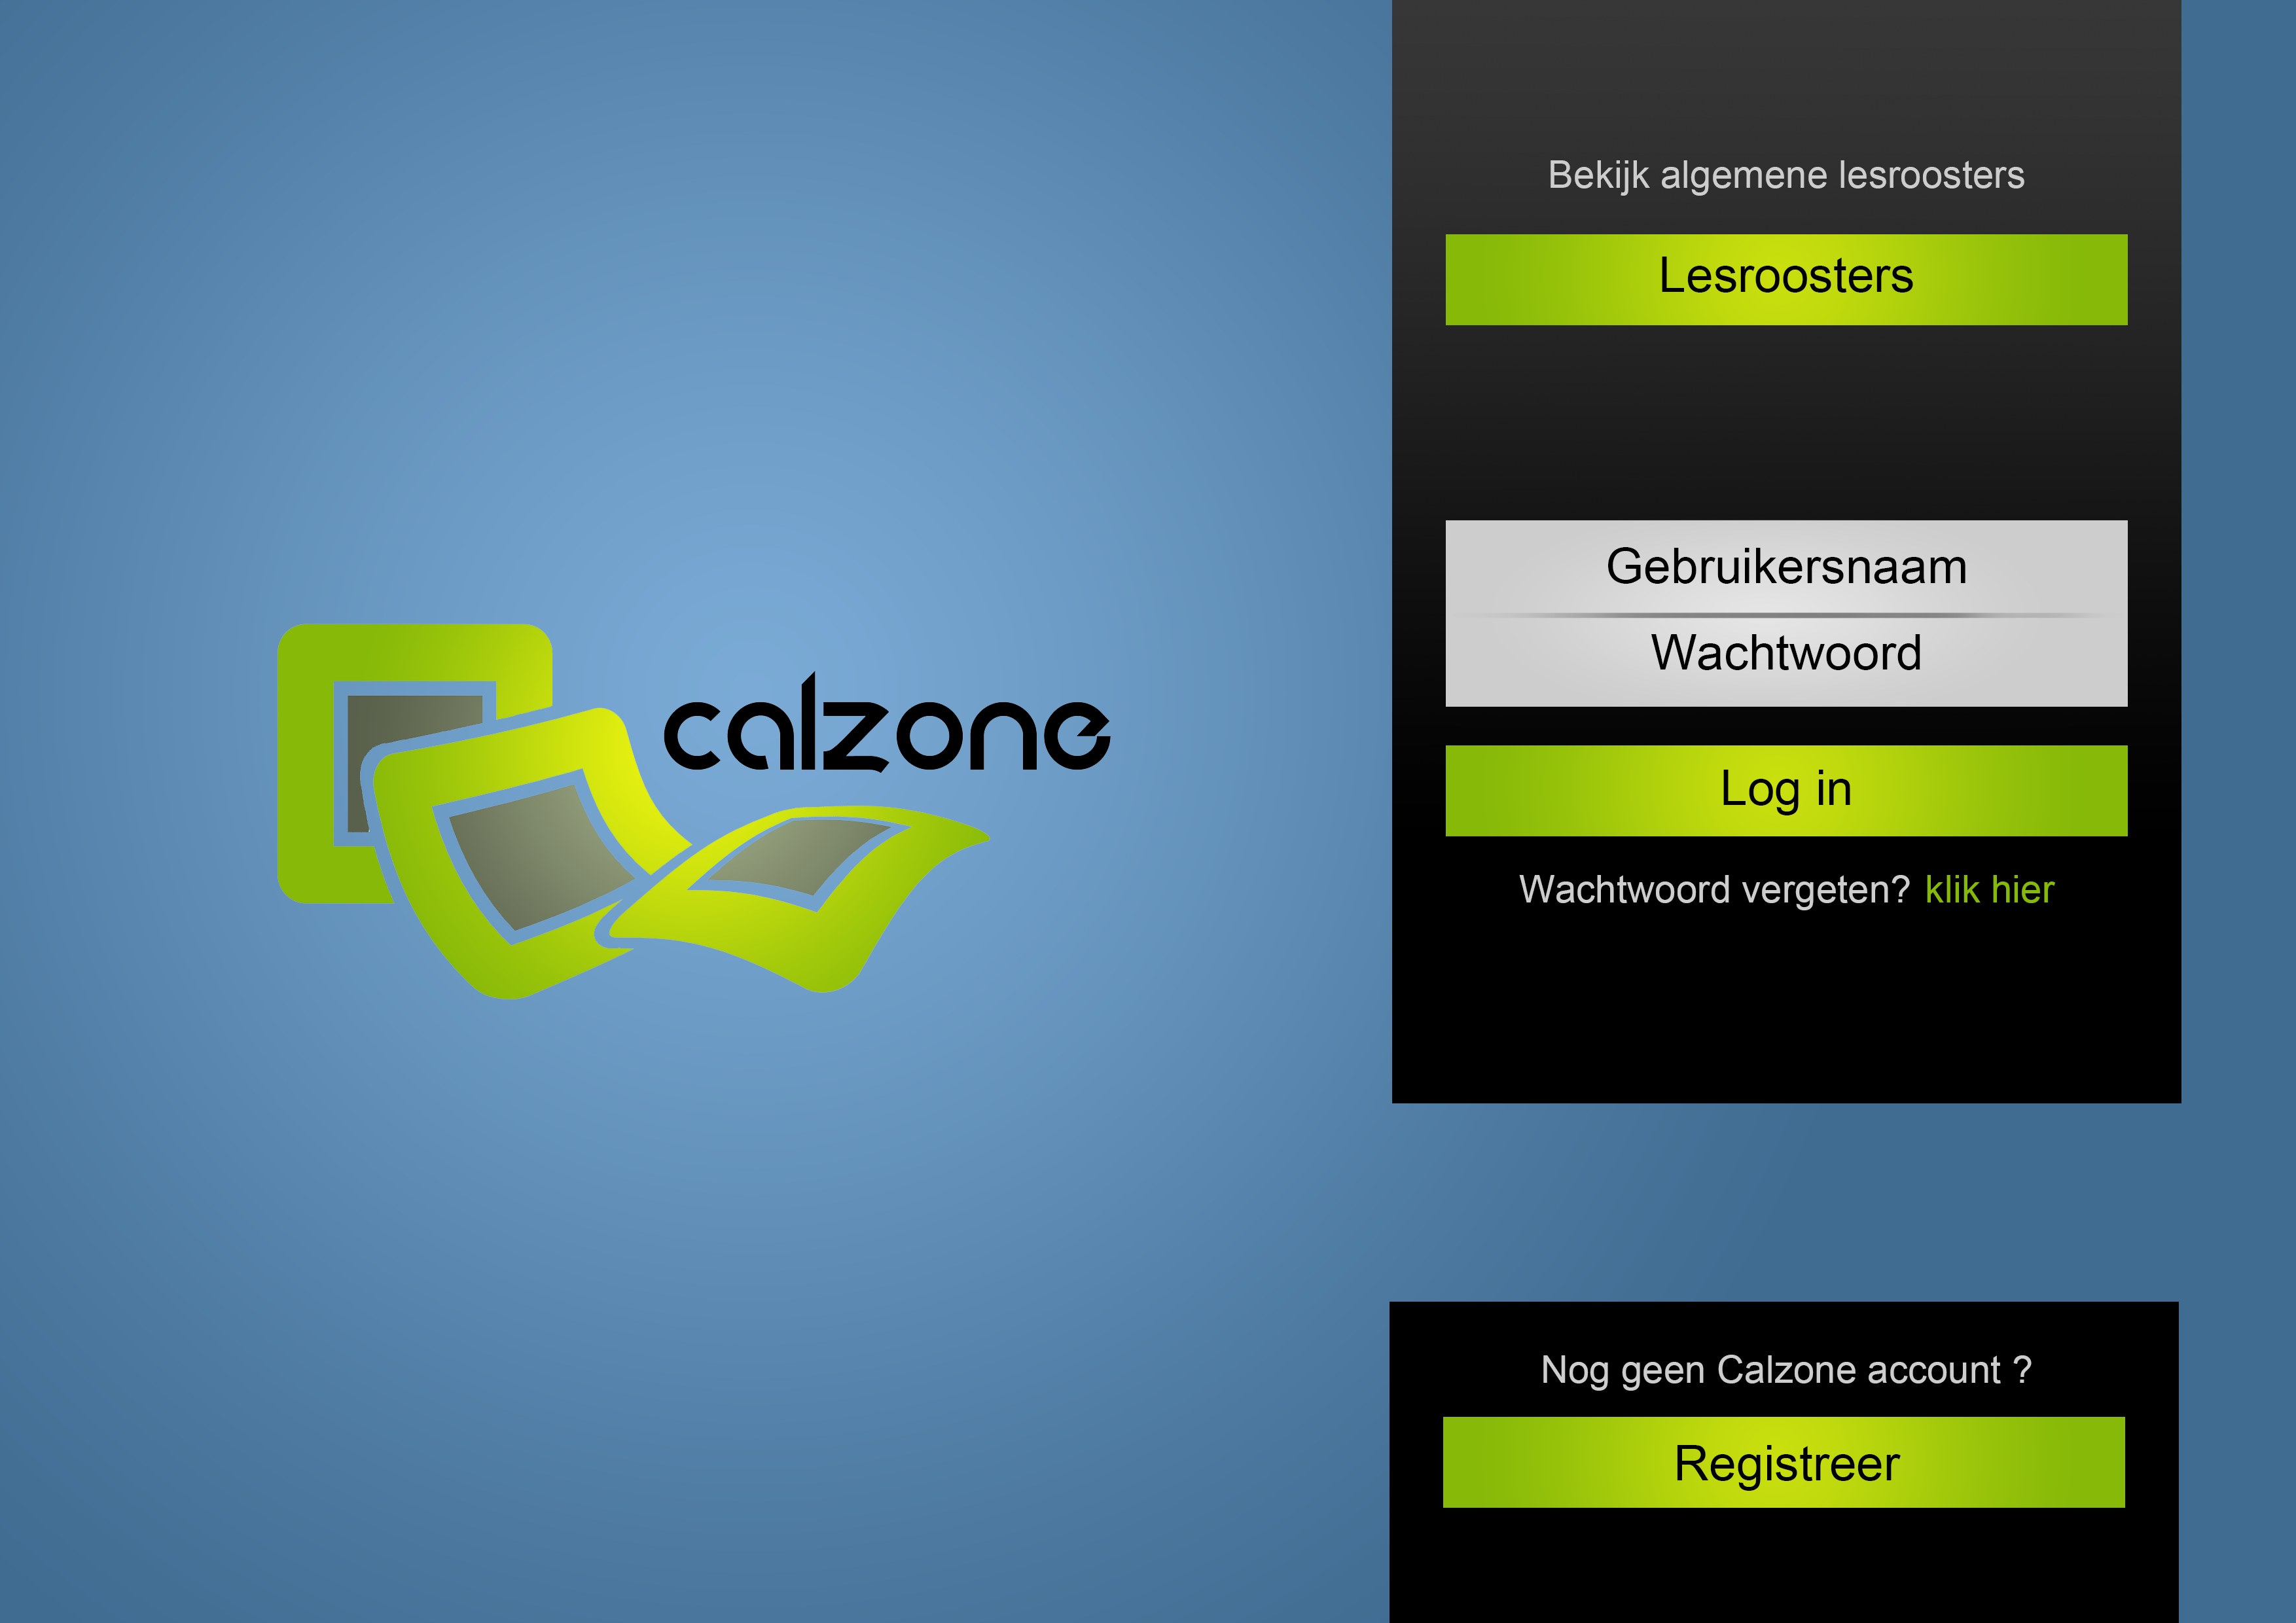
\includegraphics[scale=0.4]{img/Calzonemain}
\caption{CalZone Home}
\label{fig:CalZone Home}
\end{figure}

\begin{figure}[H]
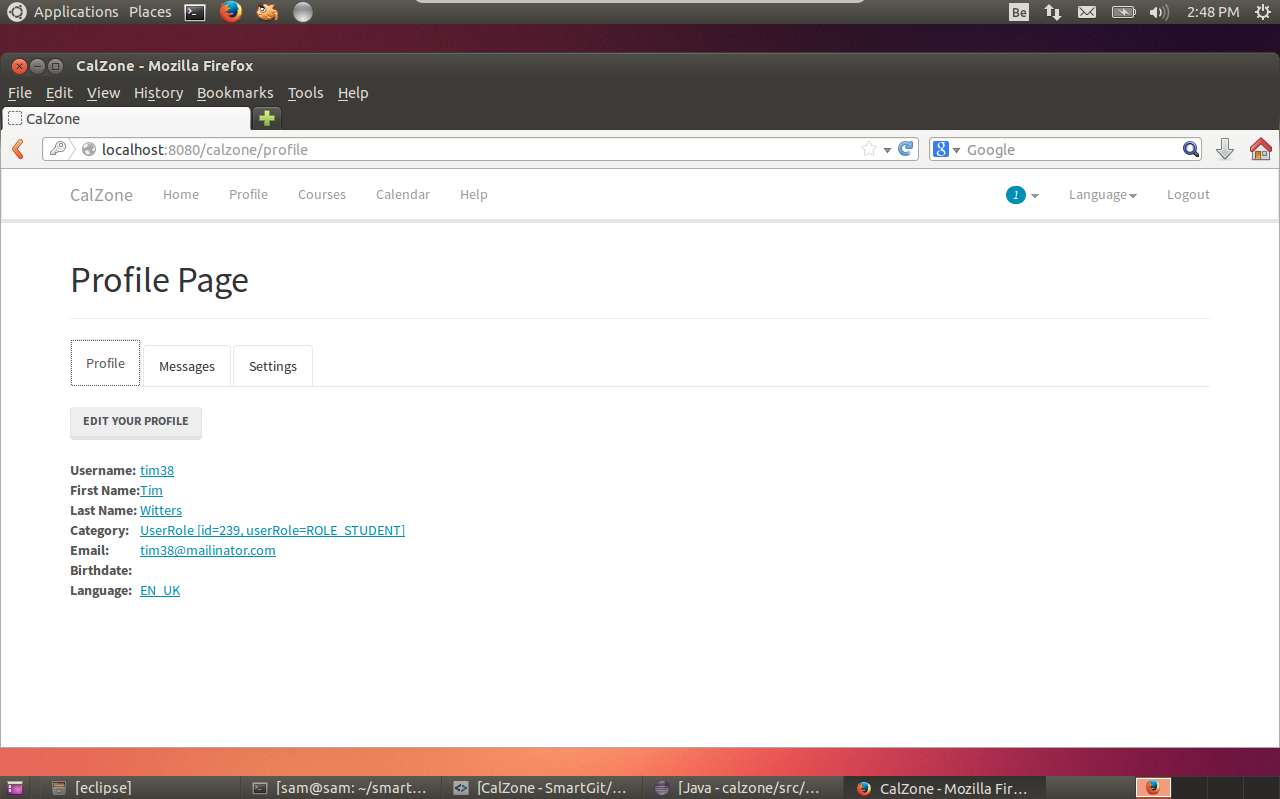
\includegraphics[scale=0.4]{img/Calzoneprofile}
\caption{CalZone Profile}
\label{fig:CalZone Profile}
\end{figure}

\begin{figure}[H]
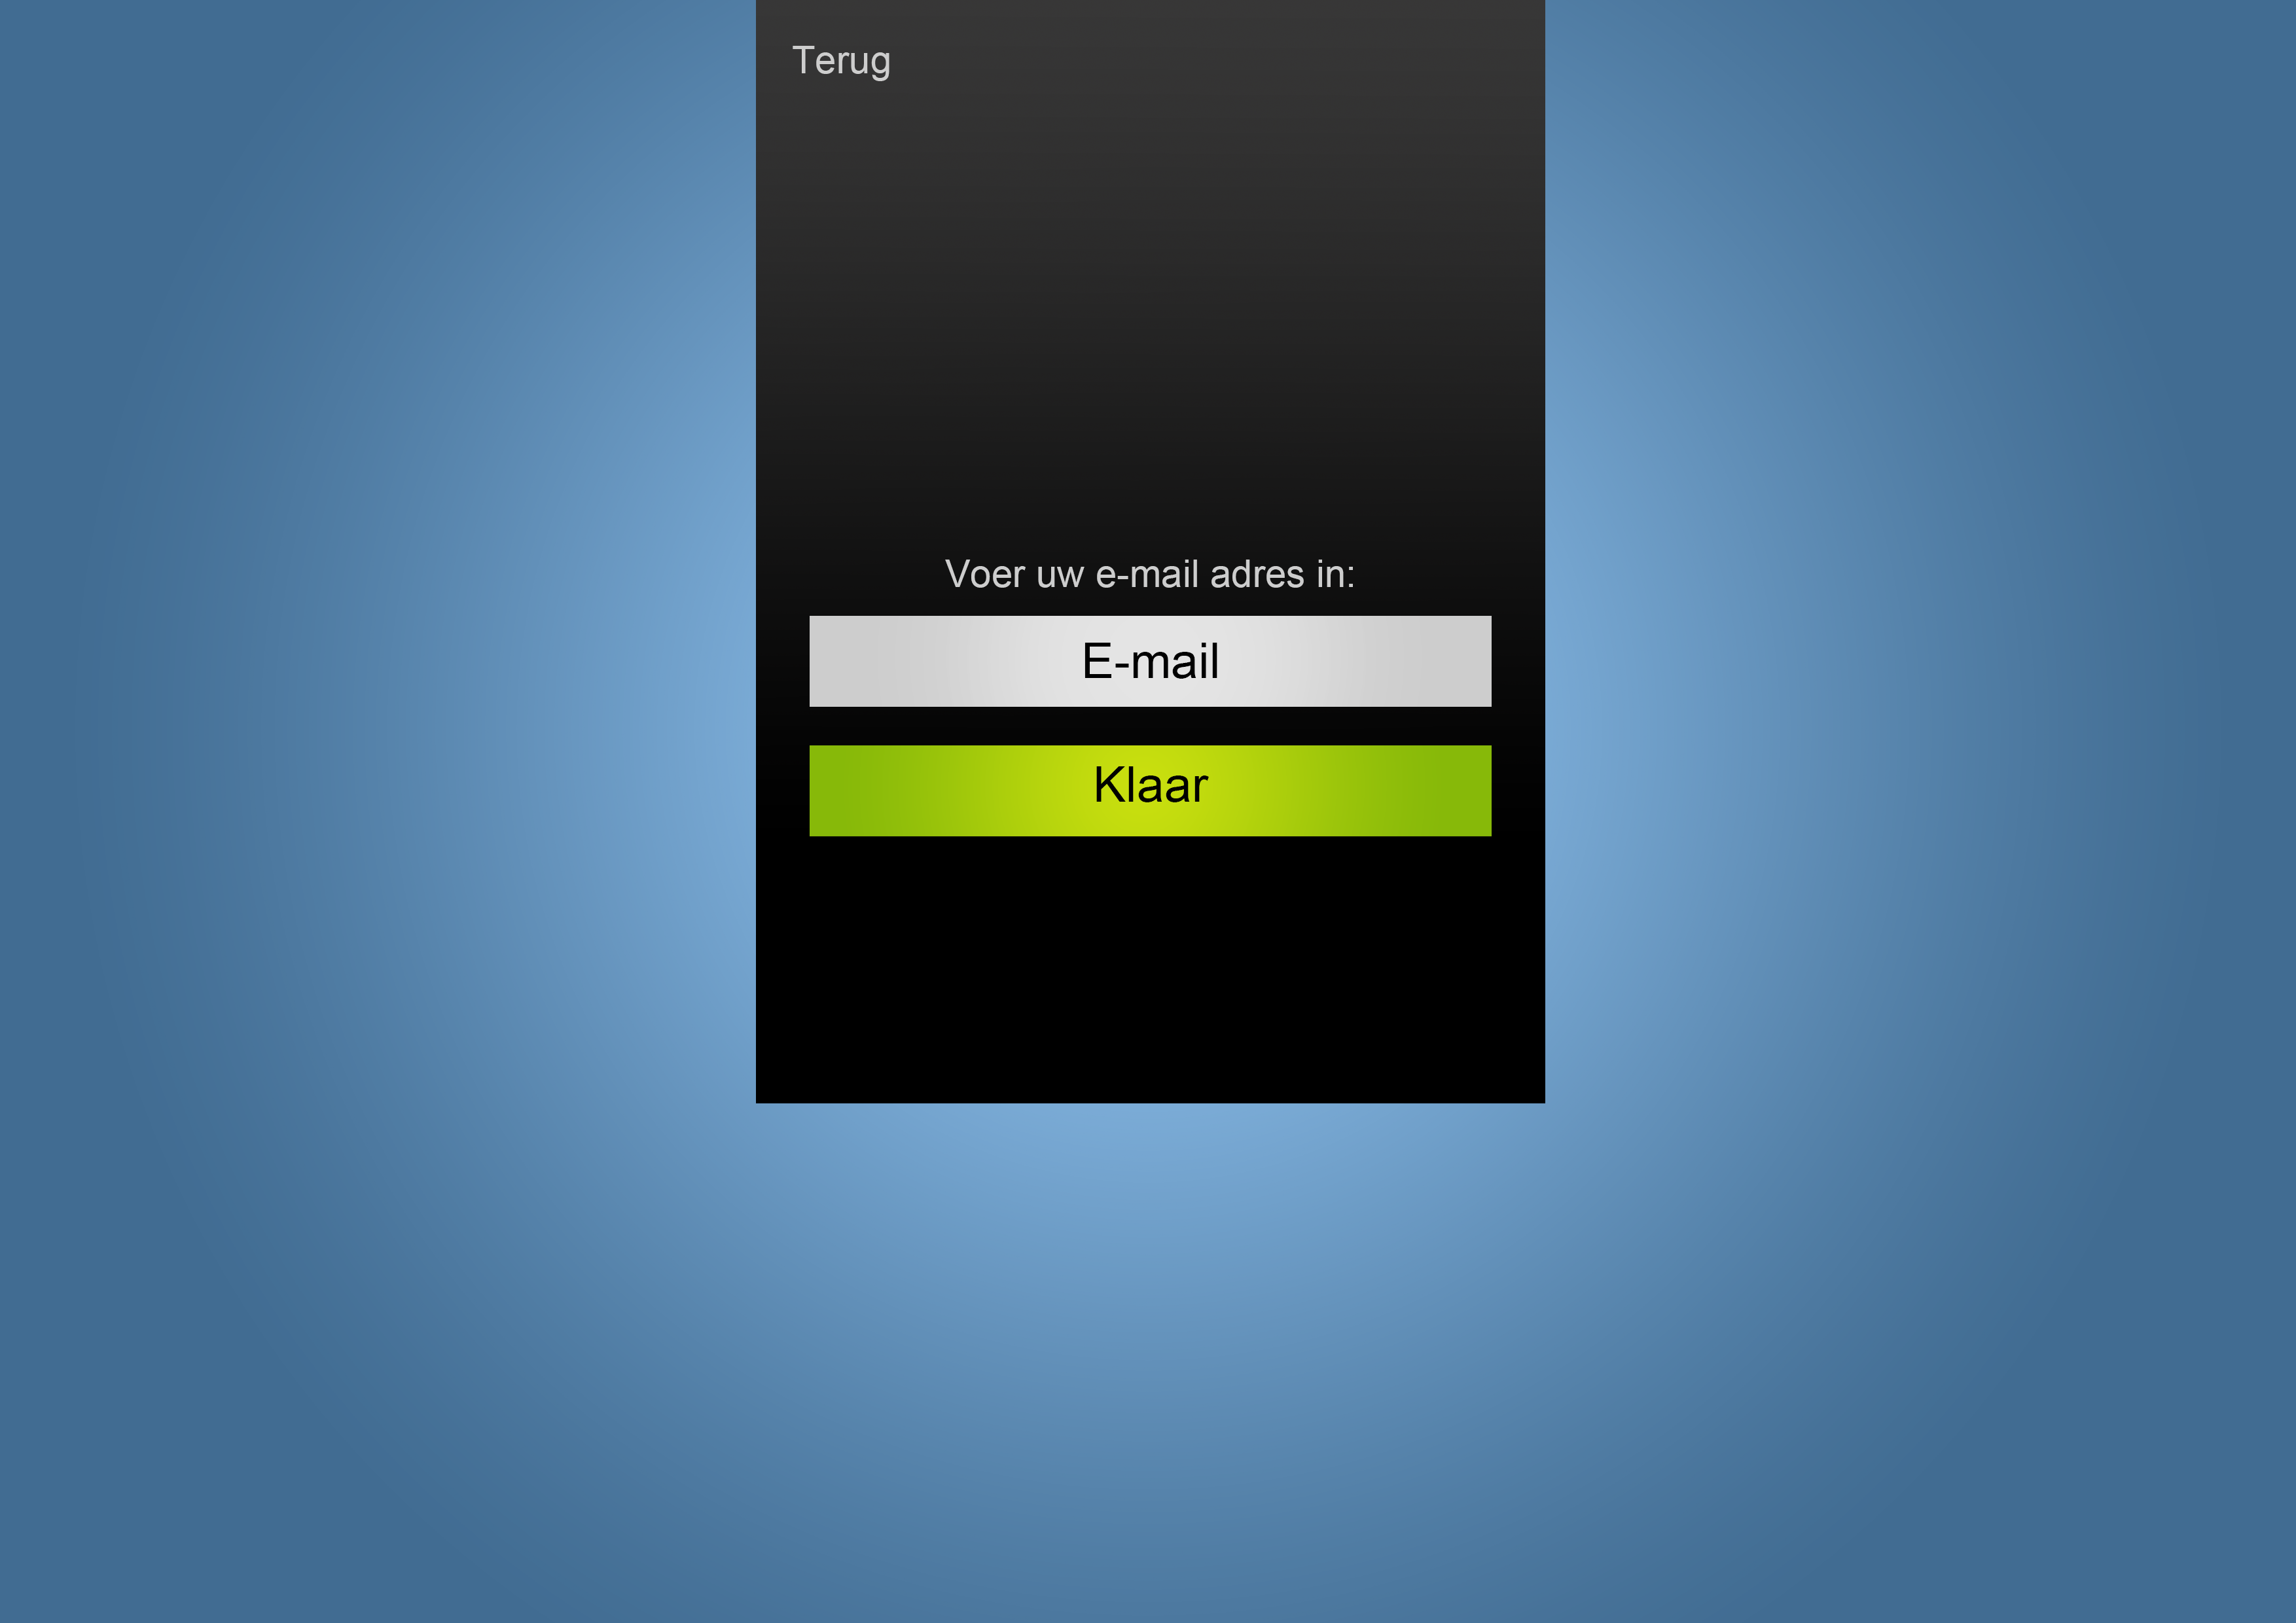
\includegraphics[scale=0.4]{img/Calzonelostpassword1}
\caption{CalZone Lost Password 1}
\label{fig:CalZone Lost Password 1}
\end{figure}

\begin{figure}[H]
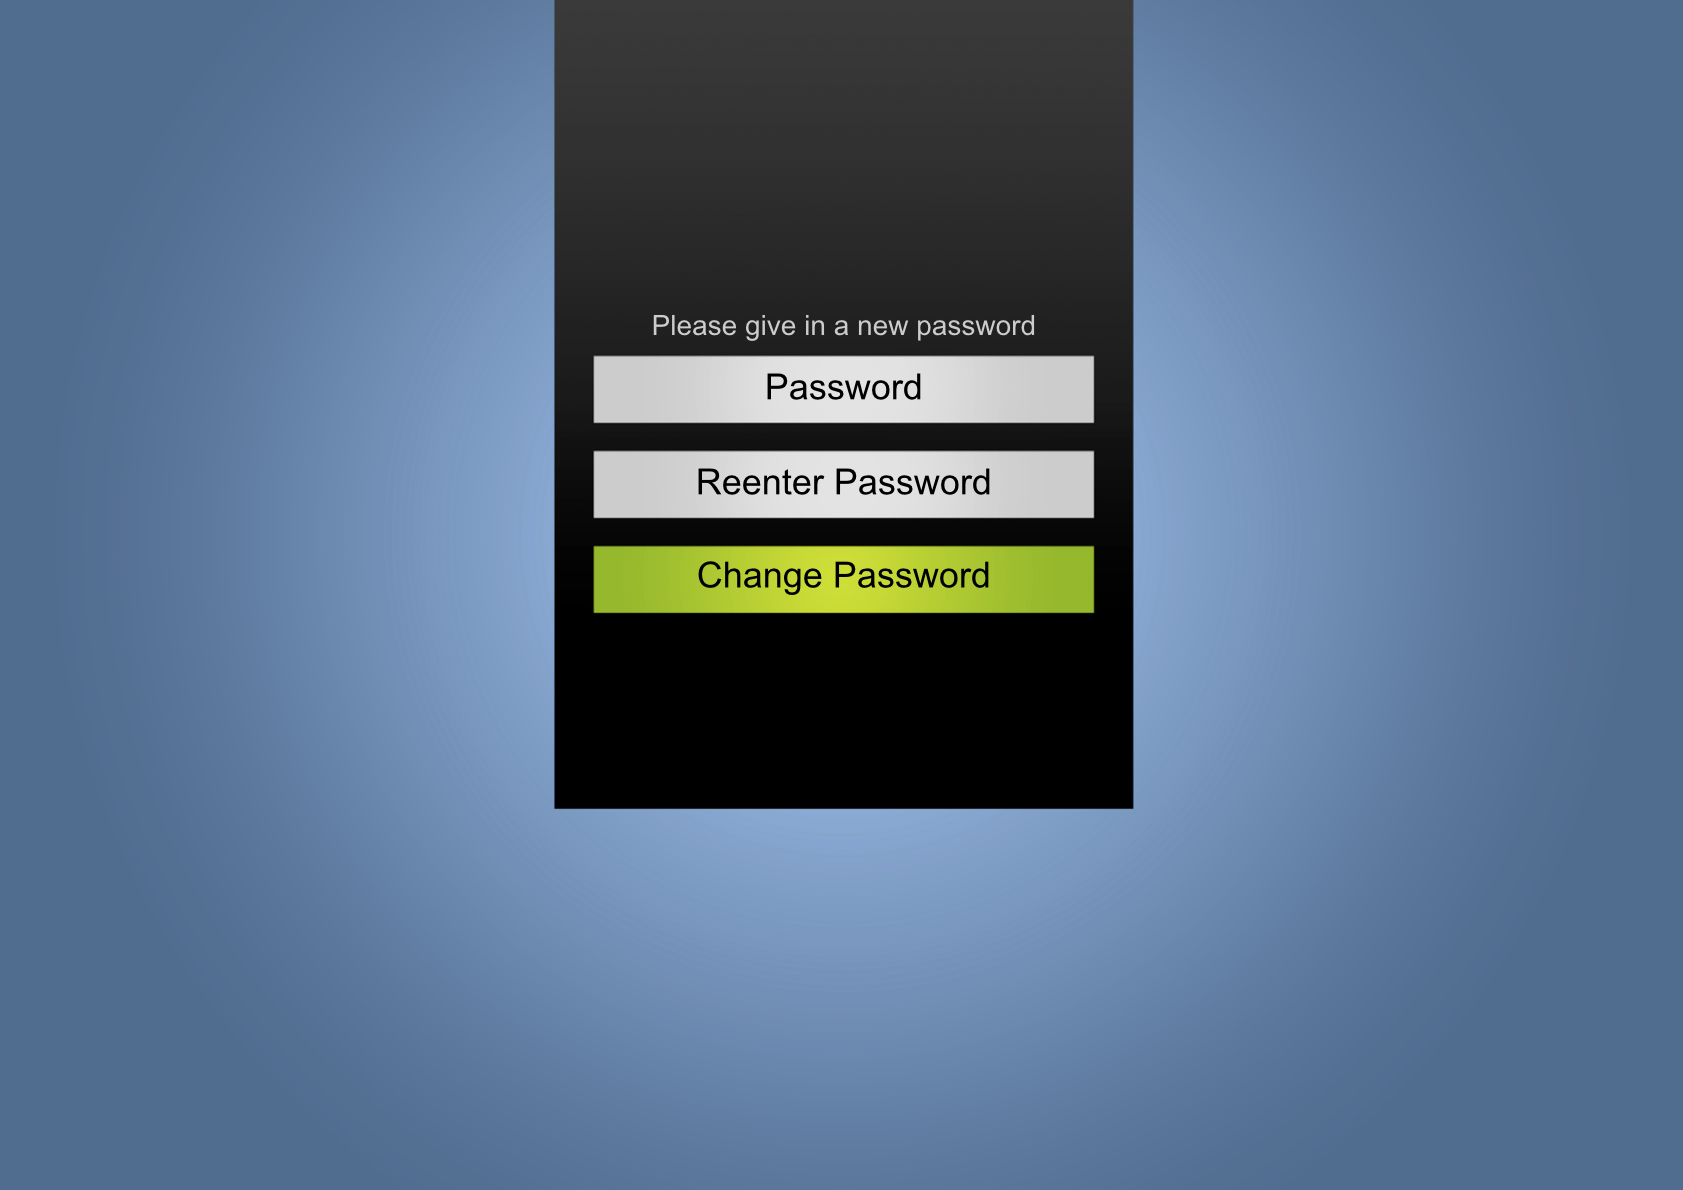
\includegraphics[scale=0.4]{img/Calzonelostpassword2}
\caption{CalZone Lost Password 2}
\label{fig:CalZone Lost Password 2}
\end{figure}

\begin{figure}[H]
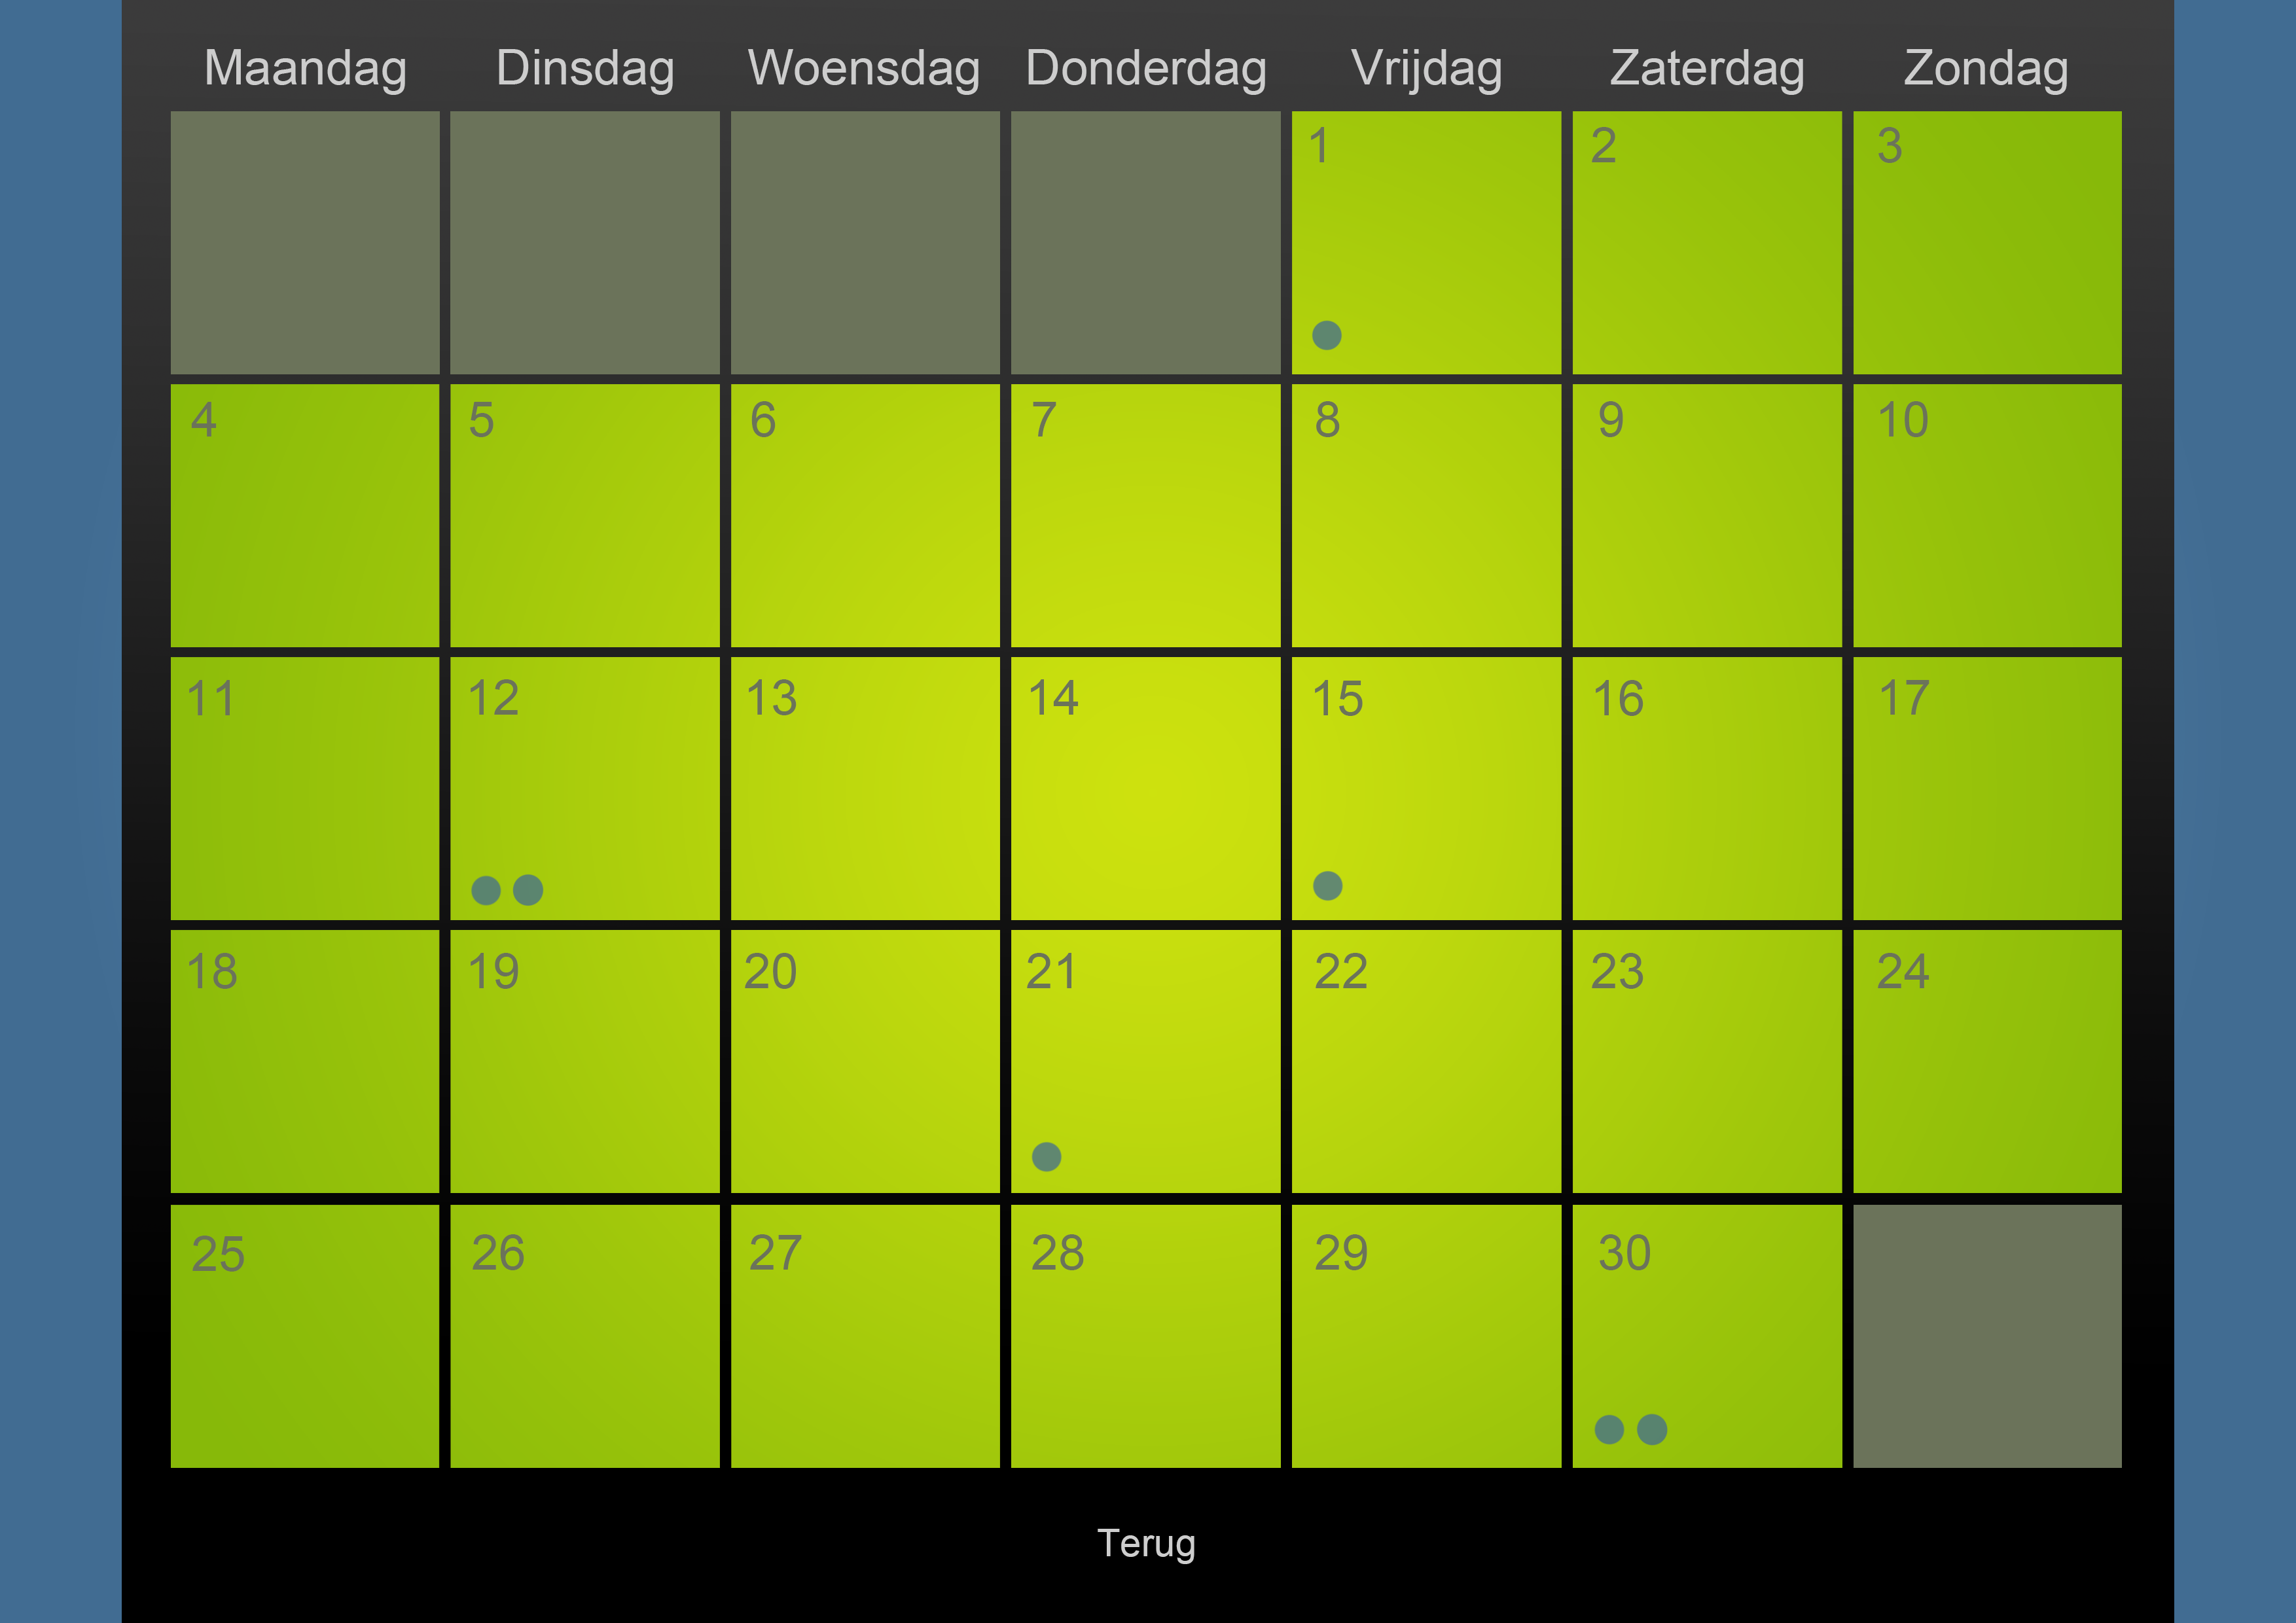
\includegraphics[scale=0.4]{img/CalzoneSchedule}
\caption{CalZone Schedule}
\label{fig:CalZone Schedule}
\end{figure}

\begin{figure}[H]
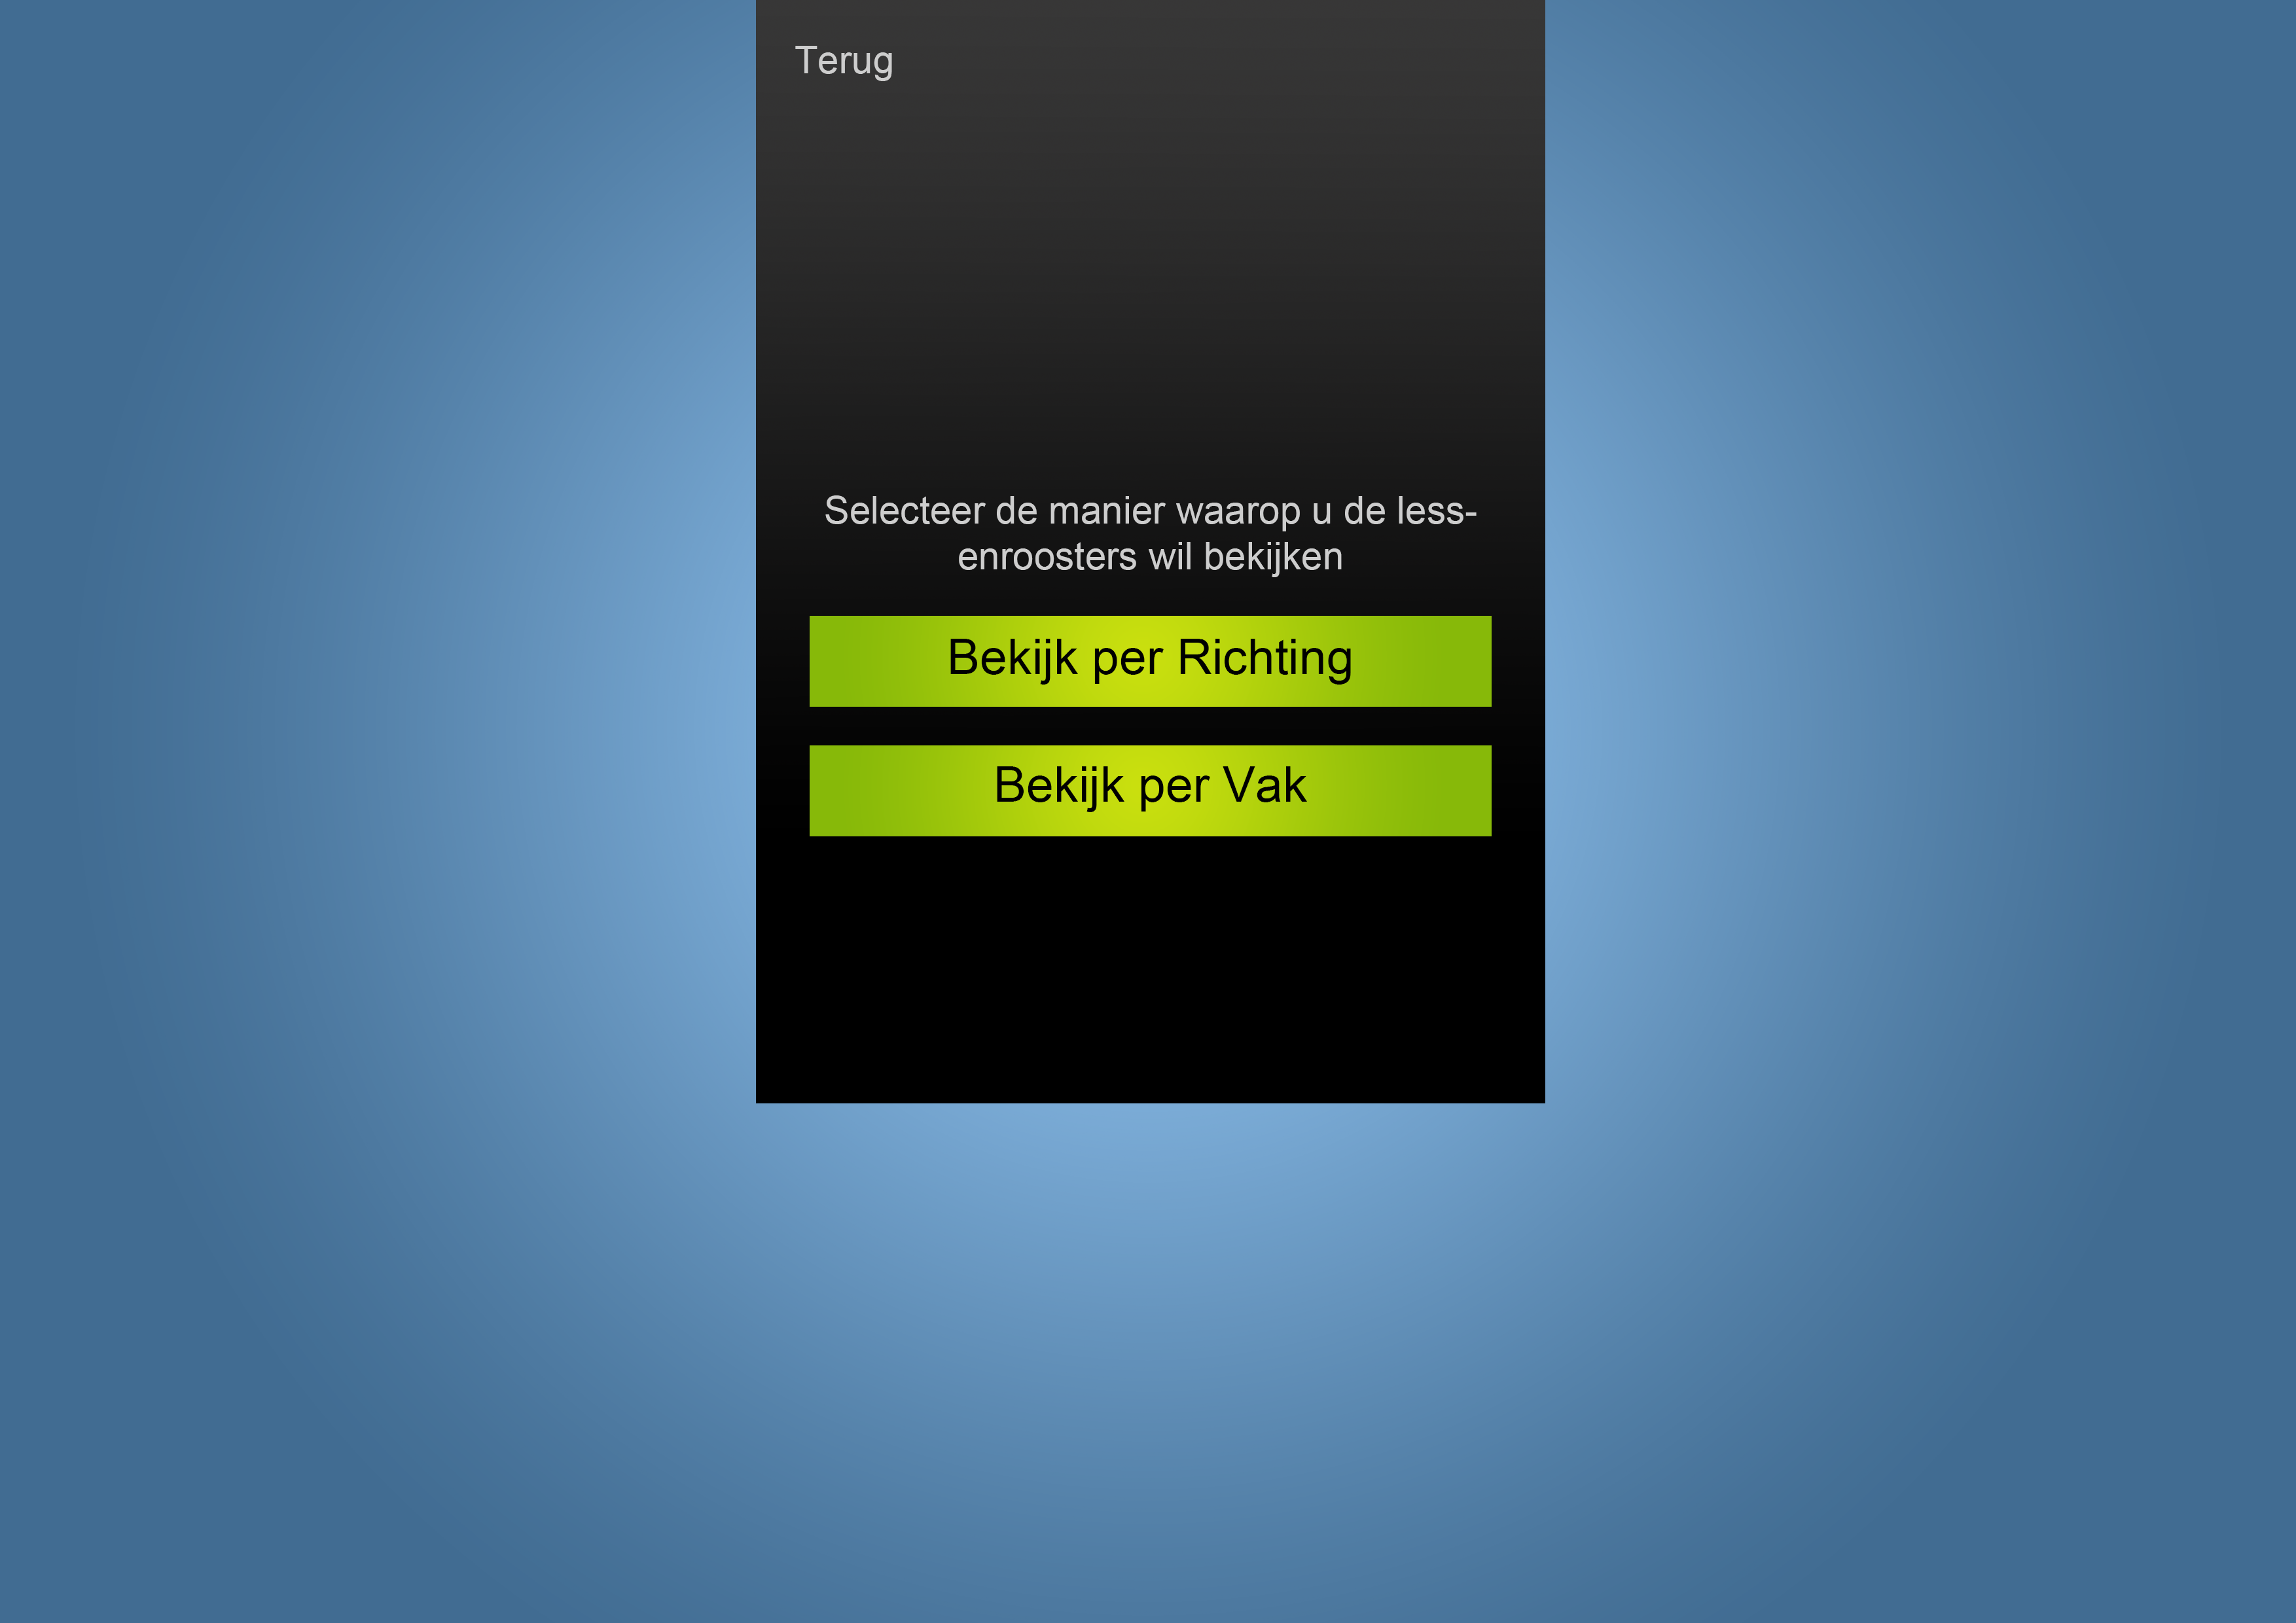
\includegraphics[scale=0.4]{img/Calzoneprogrammepicking}
\caption{CalZone Program Picking}
\label{fig:CalZone Program Picking}
\end{figure}

\begin{figure}[H]
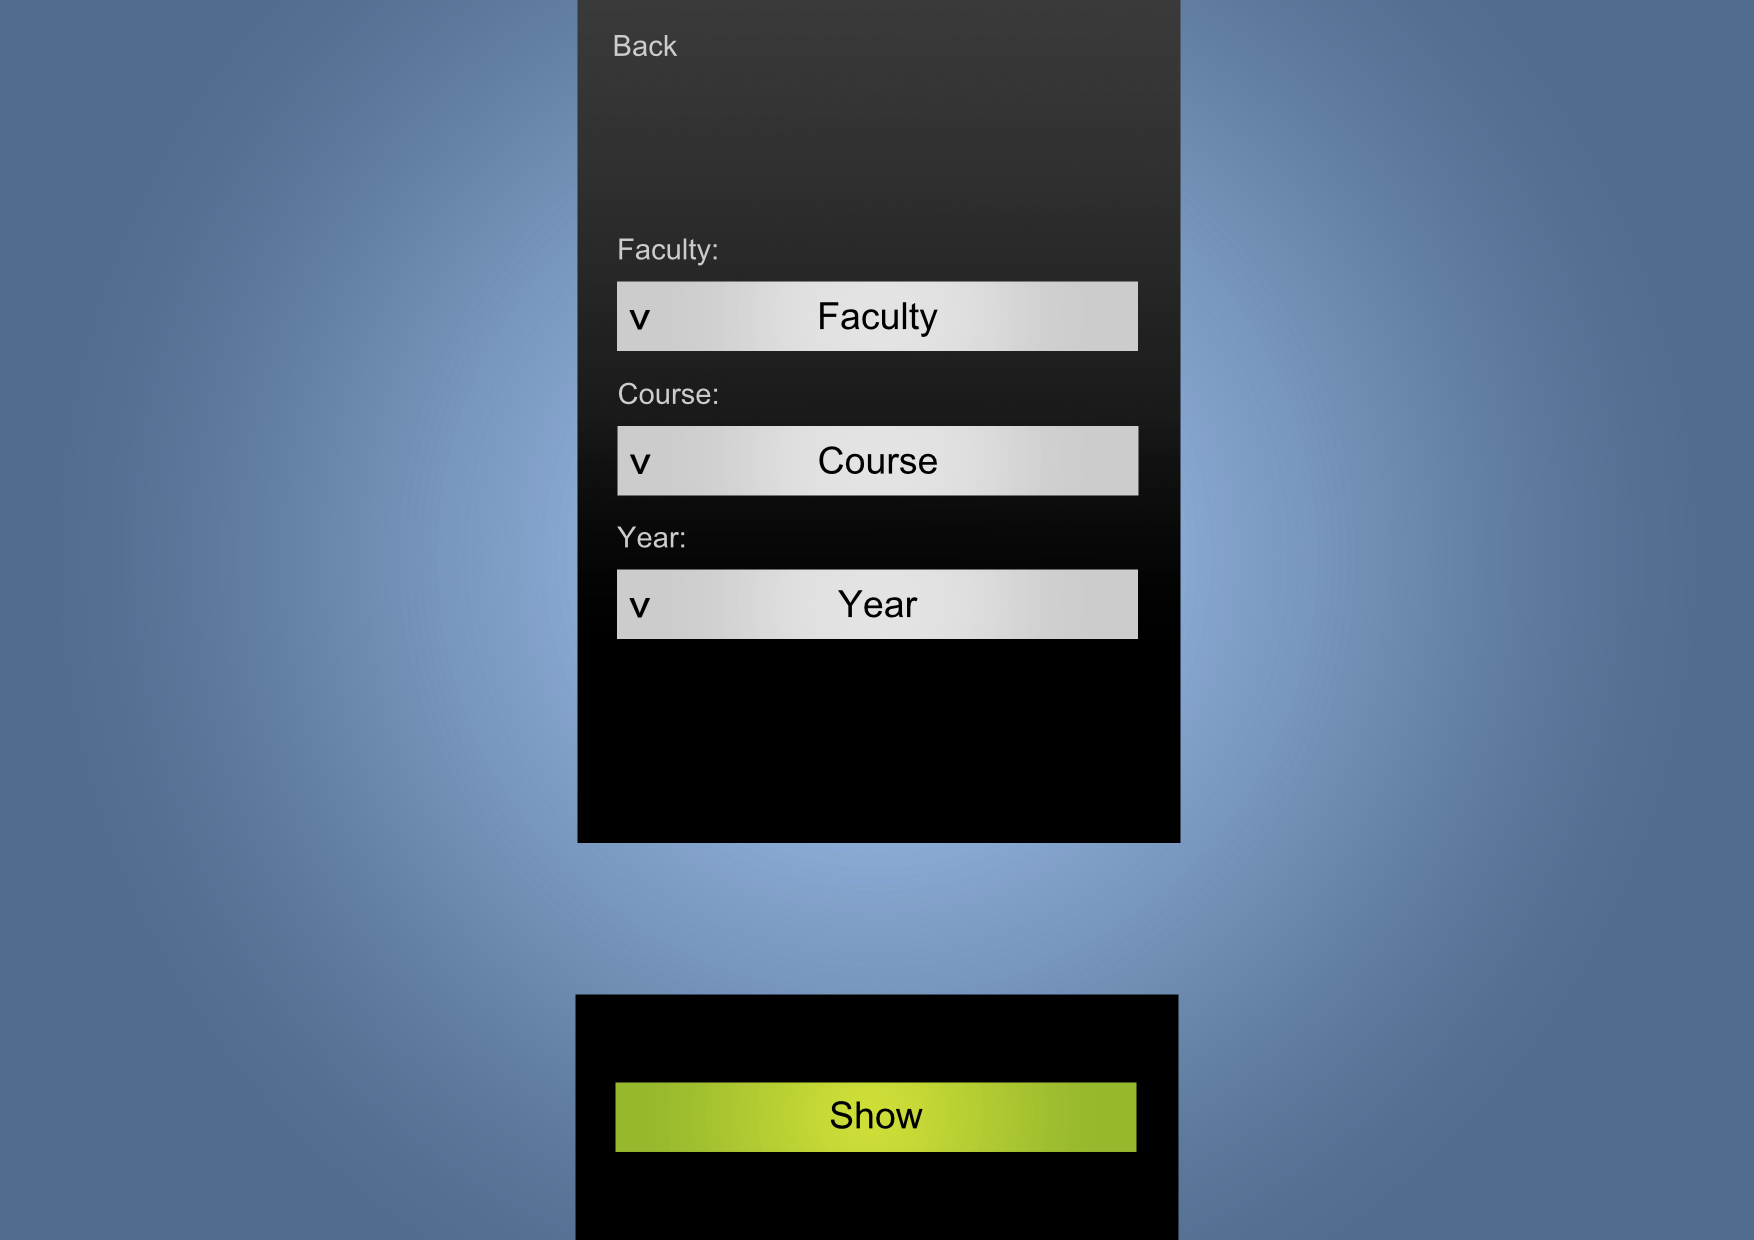
\includegraphics[scale=0.4]{img/Calzoneprogrammepicking2}
\caption{CalZone Program Picking 2}
\label{fig:CalZone Program Picking 2}
\end{figure}

\begin{figure}[H]
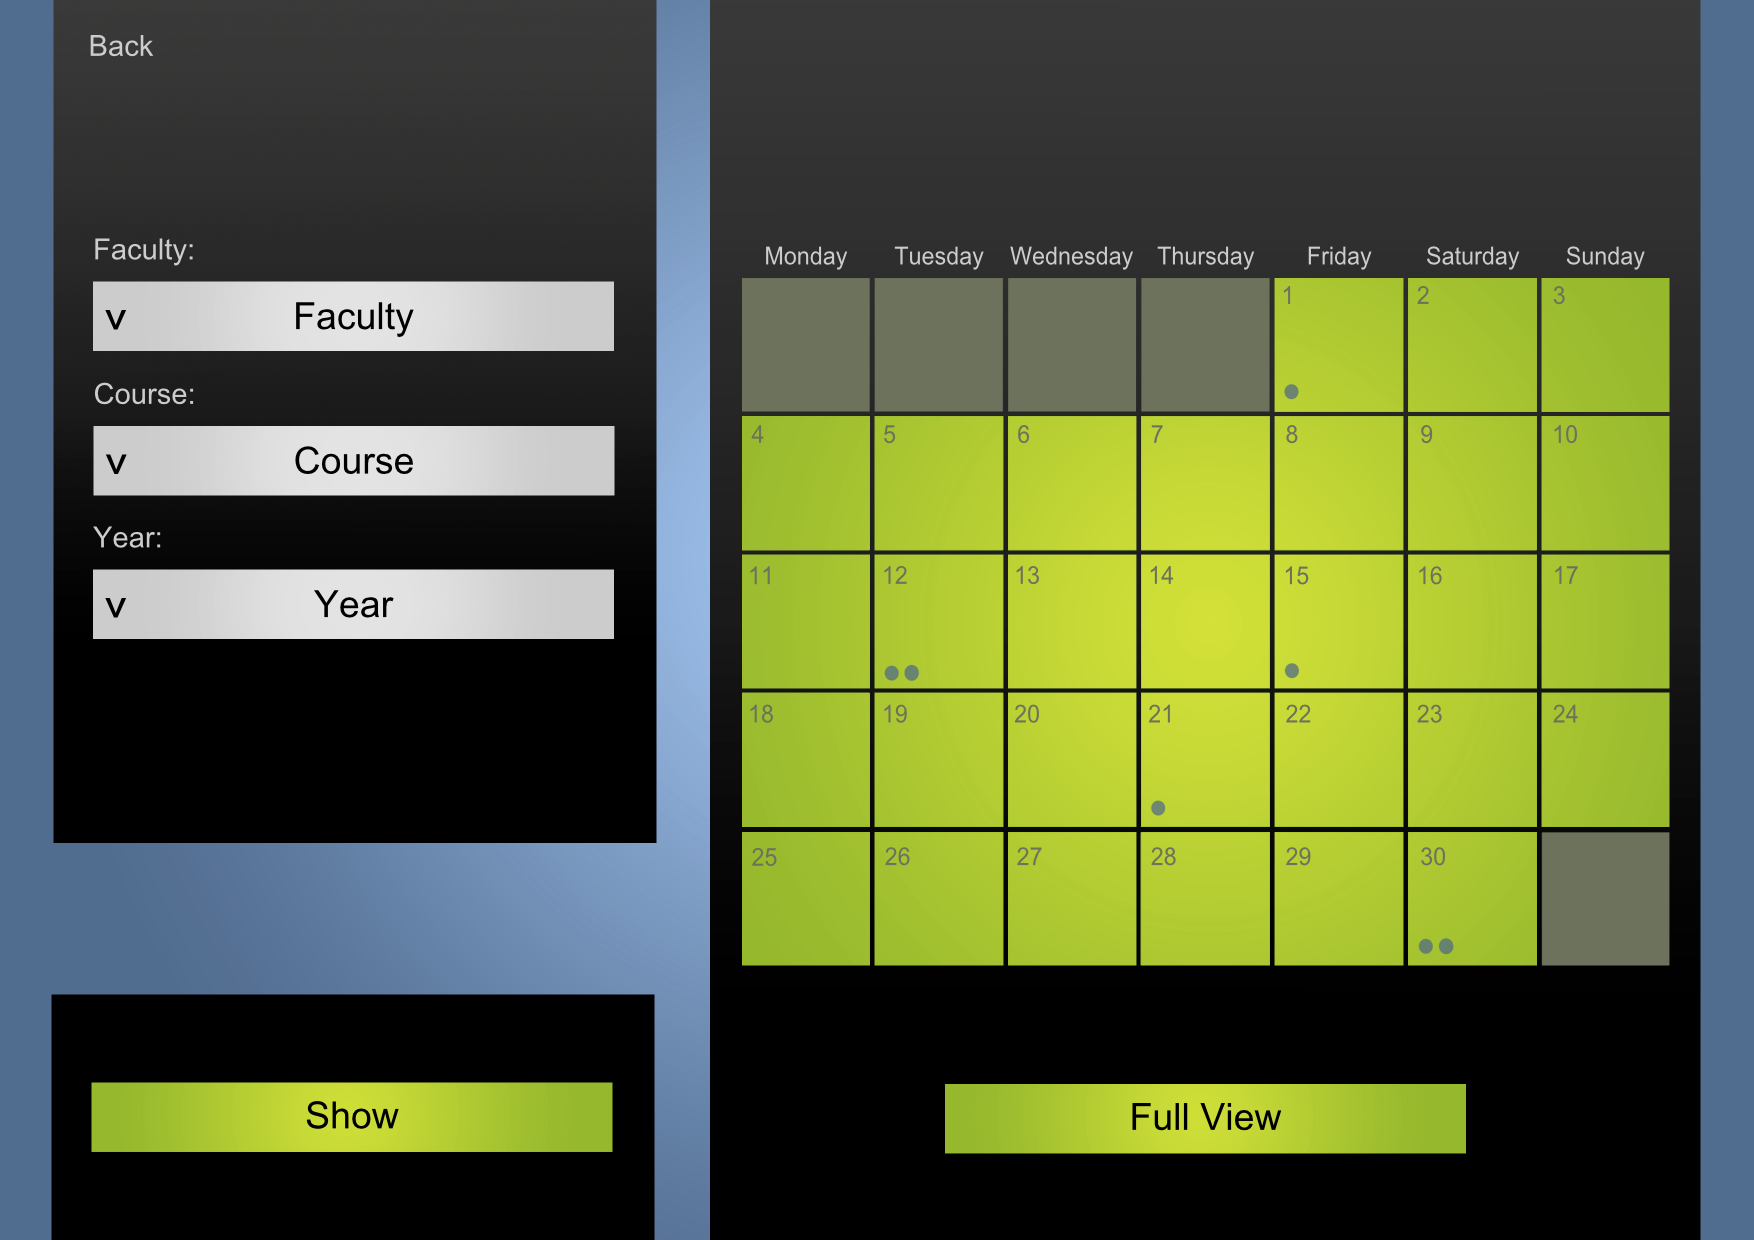
\includegraphics[scale=0.4]{img/Calzoneprogrammepicking3}
\caption{CalZone Program Picking 3}
\label{fig:CalZone Program Picking 3}
\end{figure}


\begin{figure}[H]
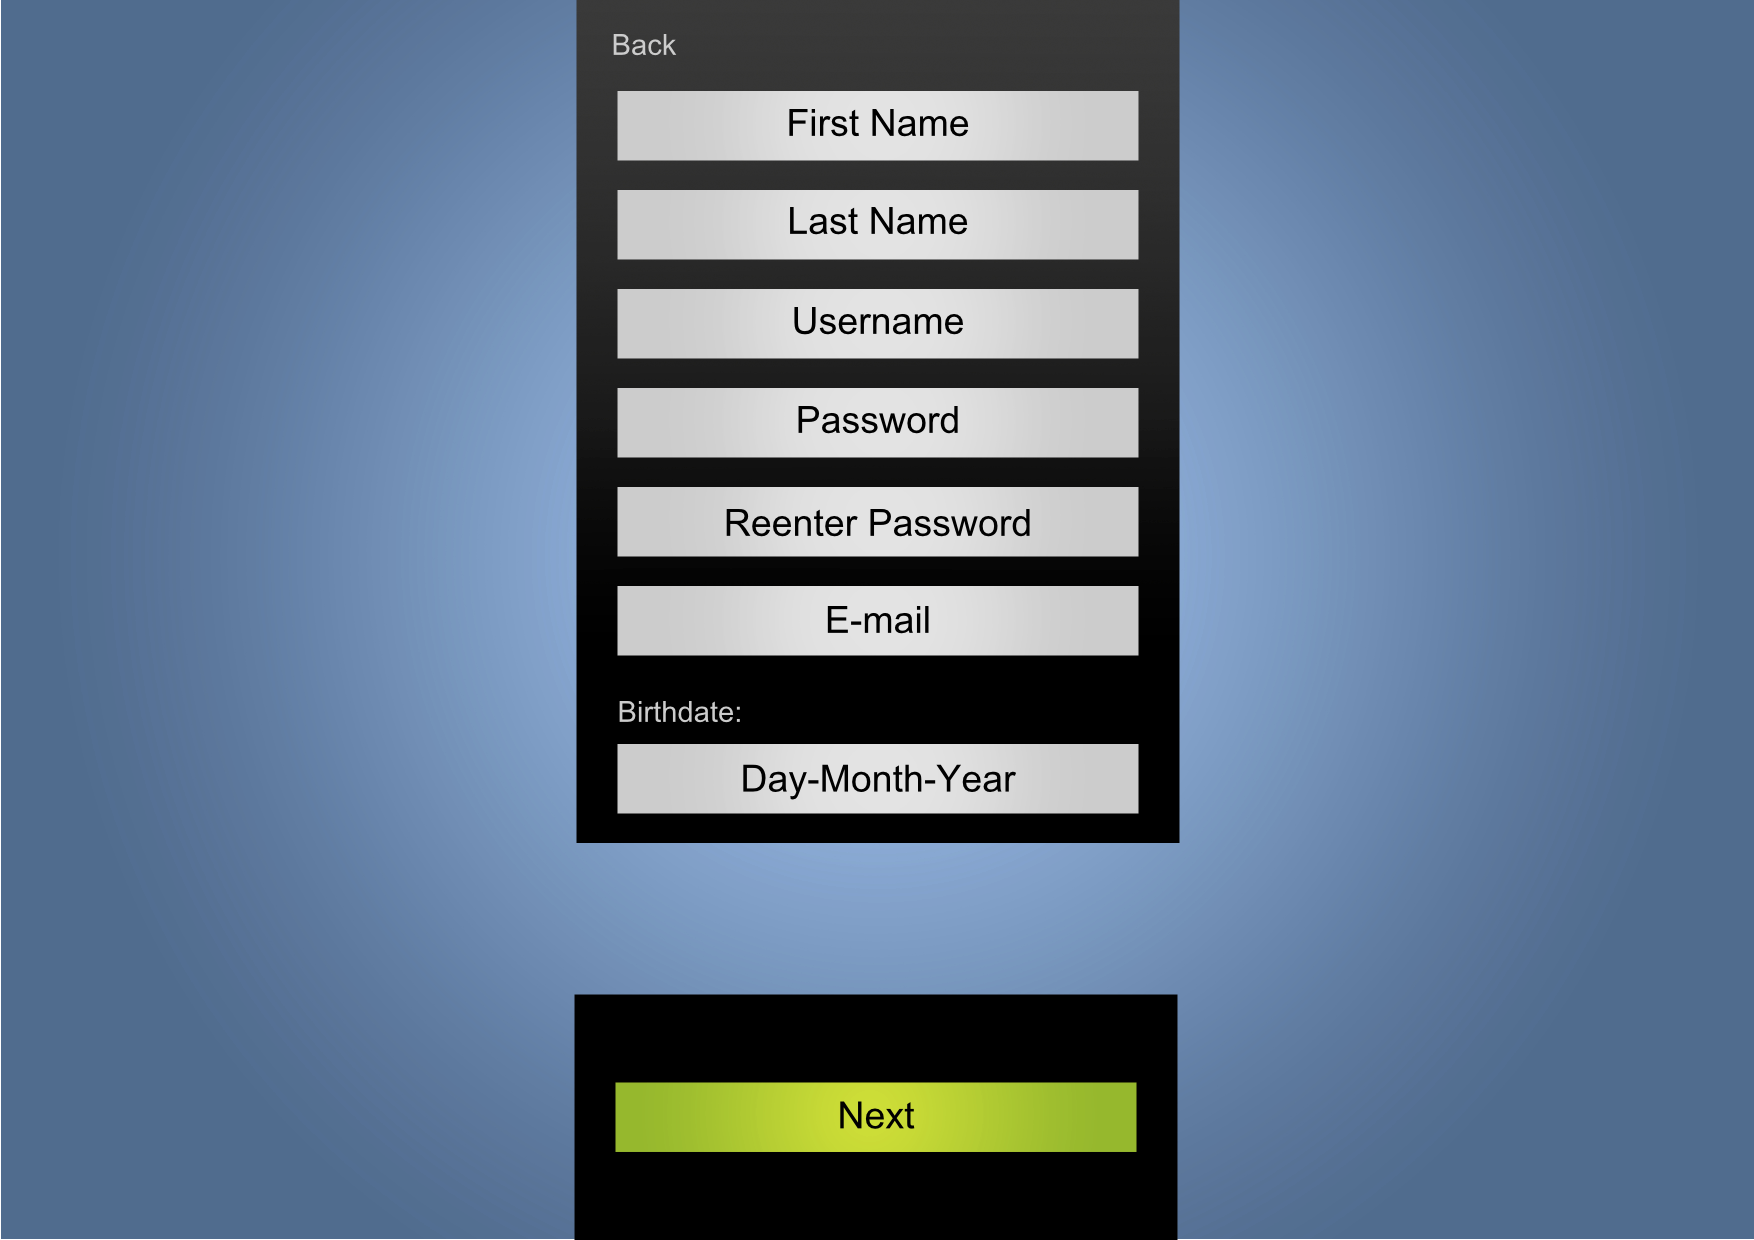
\includegraphics[scale=0.4]{img/Calzonesignup}
\caption{CalZone Program Sign Up}
\label{fig:CalZone Program Sign Up}
\end{figure}

\begin{figure}[H]
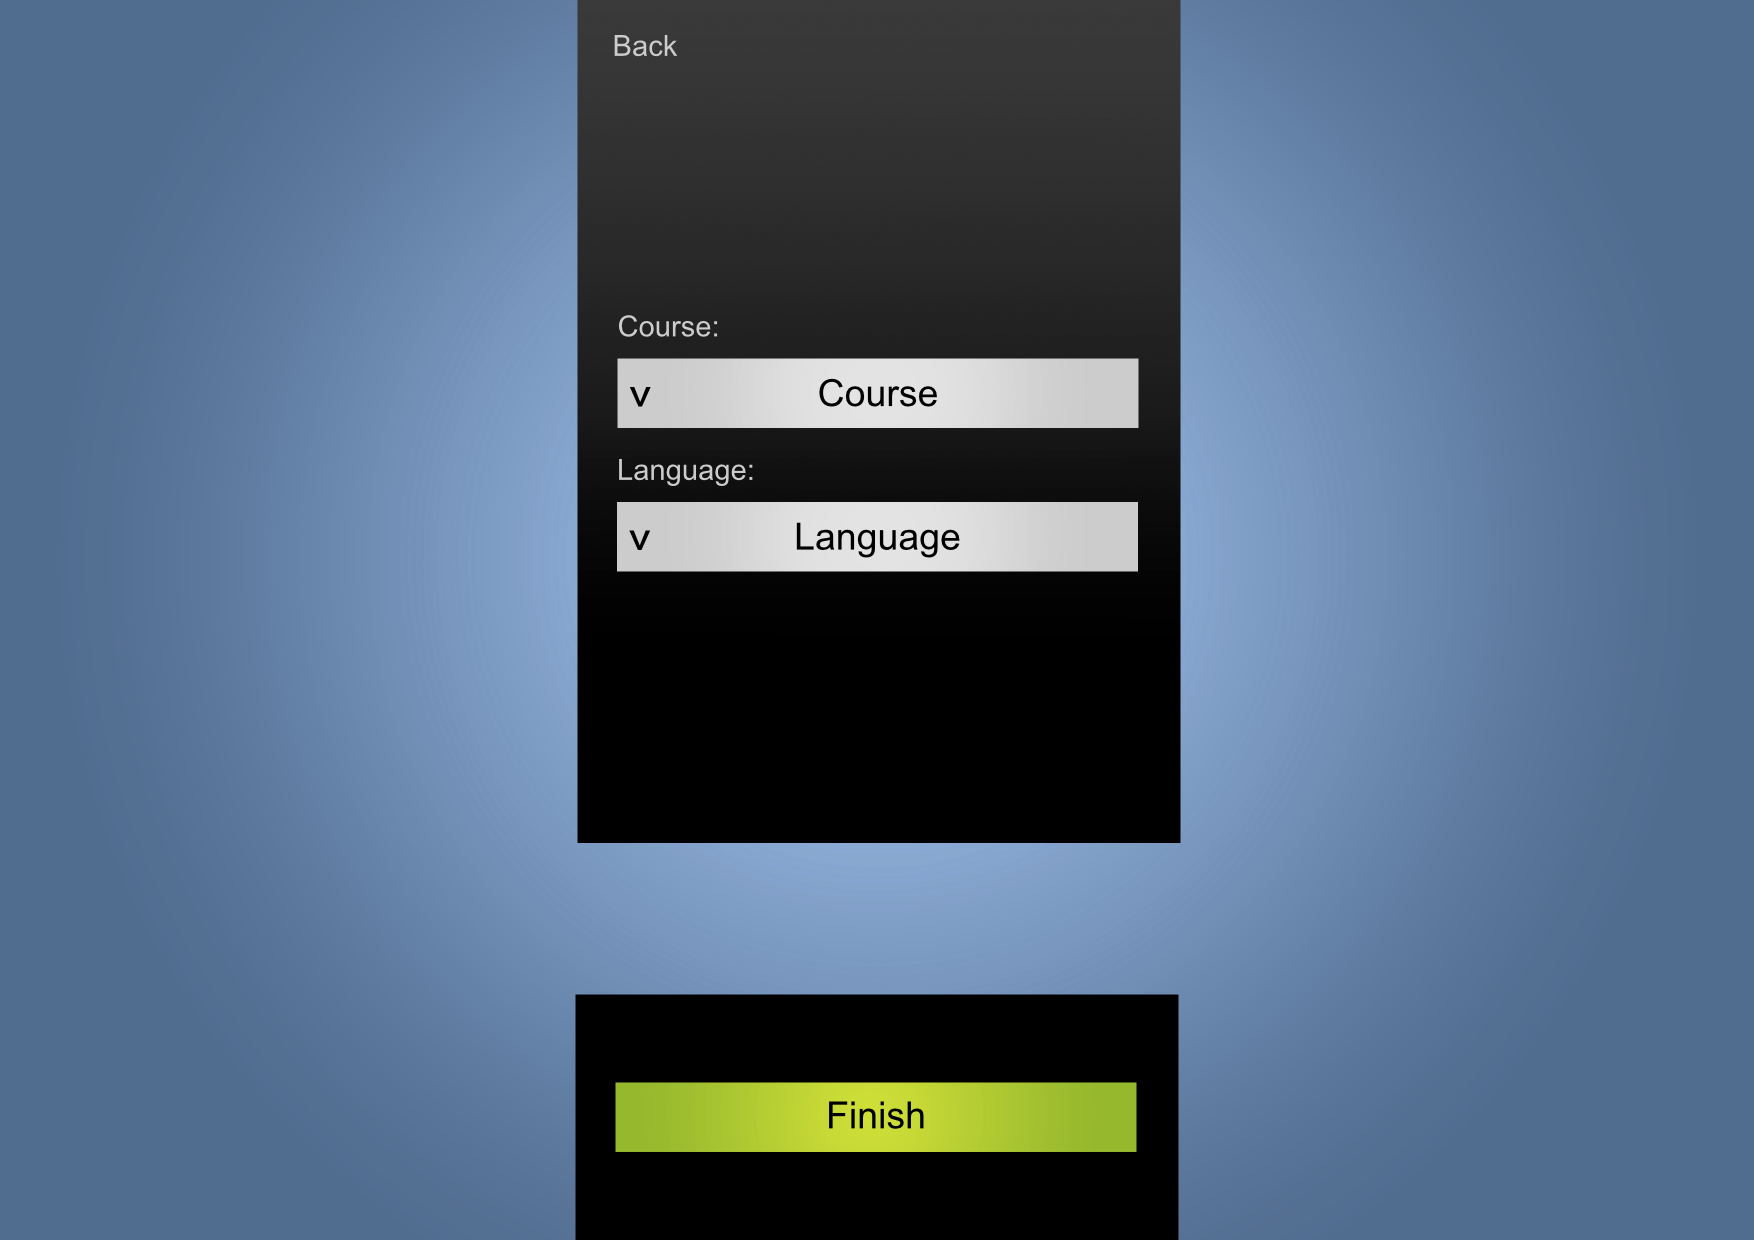
\includegraphics[scale=0.4]{img/Calzonesignup2}
\caption{CalZone Program Sign Up 2}
\label{fig:CalZone Program Sign Up 2}
\end{figure}

\end{center}
\clearpage


\section{Niet Functionele Requirements}
\subsection{Beveiliging - NFR1}

%Implementatie van HTTPS
\subsubsection{Implementatie van HTTPS}
	\begin{table}[H]
	\caption{NFR1.1 - Implementatie van HTTPS}
    		\begin{tabular}{l | p{10cm}}
        \textbf{ID:} & NFR1.1 \\ \hline
        \textbf{TITEL:} & Implementatie van HTTPS \\ \hline
        \textbf{PRIORITEIT:} &  Medium \\ \hline
        \textbf{PREREQUISITIES:} & Geen\\ \hline
        \textbf{BESCHRIJVING:} & HTTPS gebruiken voor de beveiliging van de applicatie.\\
    \end{tabular} 
	\label{tab:NFR1.1 -Implementatie van HTTPS}
\end{table}

%Hashing
\subsubsection{Hashing}
	\begin{table}[H]
	\caption{NFR1.2 - Hasing}
    		\begin{tabular}{l | p{10cm}}
        \textbf{ID:} & NFR1.2 \\ \hline
        \textbf{TITEL:} & Hashing \\ \hline
        \textbf{PRIORITEIT:} &  Hoog \\ \hline
        \textbf{PREREQUISITIES:} & Geen\\ \hline
        \textbf{BESCHRIJVING:} & Wachtwoorden moeten in de database opgeslagen worden met behulp van een hash. Er zal gebruik gemaakt worden van SHA-256 als cryptografische hash functie en een SALT.\\
    \end{tabular} 
	\label{tab:NFR1.2 -Hashing}
\end{table}

%Session Management
\subsubsection{Session Management}
	\begin{table}[H]
	\caption{NFR1.3 - Session Management}
    		\begin{tabular}{l | p{10cm}}
        \textbf{ID:} & NFR1.3 \\ \hline
        \textbf{TITEL:} & Session Management \\ \hline
        \textbf{PRIORITEIT:} &  Medium \\ \hline
        \textbf{PREREQUISITIES:} & Geen\\ \hline
        \textbf{BESCHRIJVING:} & Elke user-agent krijgt zijn eigen sessie zodat bij het uitloggen alle sessie tupels die overeenkomen met de user ID verwijderd kunnen worden.\\
    \end{tabular} 
	\label{tab:NFR1.3 -Session Management}
\end{table}



\end{document}